\section{Quark and Hadron Universe}\label{part2}
%%%%%%%%%%%%%%%%%%%%%%%%%%%%%%%%%%%%%%%%%
\subsection{Heavy particles in the QGP epoch}
\label{HiggsQGP}
%%%%%%%%%%%%%%%%%%%%%%%%%%%%%%%%%%%%
\para{Matter phases in extreme conditions}
This section will be focused on a few examples of interest to cosmological context. In the temperature domain below electro-weak (EW) boundary near $T=130$\,GeV we explore in preliminary fashion novel and interesting physical processes. We will consider the Higgs\index{Higgs}, meson, and the heavy quarks $t,b,c$ with emphasis on bottom quarks\index{bottom quark}. We will show that the bottom quarks can deviate from chemical equilibrium\index{chemical equilibrium} $\Upsilon\neq 1$ by breaking the detailed balance between production and decay reactions. It is easy to see considering temperature scaling and additional degrees of freedom that the energy density of matter near to EW phase transition is a stunning 12 orders of magnitude greater compared to the benchmark we discussed for QGP-hadronization\index{hadrons!hadronization}, see~\req{endensval}.
 
The dynamical bottom $ b,\bar b$-quark pair abundance depends on the competition between the strong interaction two gluon fusion process into $b\bar b$-pair\index{quark!bottom} and weak interaction decay rate of these heavy quarks. This leads to the off-equilibrium phenomenon of the bottom quark freeze-out in abundance near the hadronization temperature as discussed in Ref.\,\cite{Yang:2020nne} and below. Here we further argue that the same unusual situation could exist for any other heavy particle in QGP at a temperature well below their mass scale $m_h\simeq 125\GeV$. {\color{black}Note that the `official' abbreviation for the Higgs-particle is $H^0$ or subscript `H'. This conflicts with: a) The Hubble parameter in current epoch $H_0$ and with: b) The hadron gas subscript which is either `HG' or `H' in literature. Therefore in this report the Higgs-particle is abbreviated using the (subscript) symbol $h$ which has a less conflicted meaning.} We study as an example the abundance of the Higgs-particle\index{Higgs-particle} at condition $m_h\gg T$. Higgs is a particularly interesting case due to its special position in the particle ZOO and a narrow width.

We also explore the properties of hadronic phase after hadronization with special emphasis on gaining an understanding about the strangeness $s,\bar s$ content of the Universe which persists to unexpectedly low temperature. Many of the methods we use in this context were developed in order to understand the properties of strongly interacting QGP formed in relativistic \ie\ high-energy heavy-ion\index{heavy-ion!collisions} \ie\ nuclear collision experiments. Such experimental program is in progress at the Relativistic heavy-ion Collider (RHIC) at BNL-New York\index{BNL!RHIC} and the Large Hadron Collider (LHC) at CERN\index{CERN!LHC}. 

Let us remind the reasons why the dynamics of particles and plasma in the primordial Universe differs greatly from the laboratory environment. We focus here on the case of QGP-hadron phase boundary but a similar list applies to other era boundaries:\index{Big-Bang!micro-bang comparison}
\begin{enumerate} 
\item The primordial Big-Bang QGP epoch lasts for about $20\,\mu$s. On the other hand, the QGP formed in collision micro-bangs has a lifespan of around $10^{-23}$\,s. 
\item In the primordial Universe the microscopic transformation of quarks into hadrons proceeded through creation of the so called mixed phase allowing for local equilibration and a full relaxation of strongly interacting degrees of freedom during about $10\,\mu$s~\cite{Fromerth:2002wb}. Contemporary lattice QCD model simulations predict a smooth transformation as well. The transformation in the laboratory is much closer to what can be called explosive and sudden conversion of quarks into hadronic (confined) degrees of freedom~\cite{Rafelski:2000by}. Such a situation can mimic phenomena usually observed in a true phase transition of first order.
\item Half of the degrees of freedom present in the Universe (charged leptons, photons, neutrinos) are not part of the thermal laboratory micro-bang.
\item Experimental reach today is at and below $T\simeq 0.5$\,GeV allowing us to explore the hadronization process of the QGP but not the heavy particle (h,W,Z,$t$) content, $b$ and $c$ quarks are difficult to study. 
\item Though the baryon content of the laboratory QGP is very low it is probably also much higher compared to the observed baryon asymmetry\index{baryon!asymmetry} in the Universe. 
\end{enumerate}
 
%%%%%%%%%%%%%%%%%%%%%%%%%%%%%%%%%%%
\para{Higgs equilibrium abundance in QGP} 
We would like to show that it is of interest to study the Higgs\index{Higgs} particle dynamics at a relatively late stage of Universe evolution. This is an ongoing project which is described here for the first time. We are now considering in the primordial Universe the temperature range $10\,\mathrm{GeV}>T>1\,\mathrm{GeV}$, and recall the mass of the Higgs-particle $m_h\simeq 125\GeV$. Therefore the number density of the Higgs can be written using the relativistic Boltzmann\index{Boltzmann!approximation} approximation
\begin{align}\label{DensityH}
n_{h}=\frac{\Upsilon_h}{2\pi^2}T^3W(m_h/T)\,\qquad W(m_h/T)=\left(\frac{m_h}{T}\right)^2 K_2(m_h/T)
\end{align}\index{Higgs!particle abundance}
where $K_2$ is the modified Bessel function of integer index '$2$'.

We are interested in comparing the abundance of the Higgs-particle to the net abundance of baryon excess over antibaryons\index{baryon!antibaryon} to determine at which temperature the Higgs-particle yield drops below this tiny Universe asymmetry. Our interest derives from the question how far down in temperature a baryon number breaking Higgs-particle decay could be of relevance. Clearly, once the Higgs-particle yield falls far below baryon asymmetry yield it would be difficult to argue that Higgs-particle sourced mechanism can contribute to a significant growth of the baryon asymmetry in the Universe. Moreover, comparing to baryon asymmetry provides in our opinion a good measure of general physical relevance. After all, our present Universe structure derives from this small asymmetry, probably developed in the primordial epoch we explore here. 
 
The density between Higgs and baryon asymmetry (quark-antiquark asymmetry) can be written normalizing to ambient entropy density
\begin{align}
\frac{n_h}{(n_B-n_{\bar{B}})}=\frac{n_{h}}{\sigma_{tot}}\,\left(\frac{\sigma_{tot}}{n_B-n_{\bar{B}}}\right)=
\frac{n_{h}}{\sigma_{tot}}\left[\frac{\sigma_{\gamma,\nu}}{n_B-n_{\bar{B}}}\right]_{t_0}\,.
\end{align}
Assuming there is no `late' baryon genesis and entropy conserving Universe expansion, we introduce in \req{BaryonEntropyRatio} in the last equality the present day value of the baryon per entropy ratio\index{baryon!entropy ratio}. The entropy density\index{entropy!density} $\sigma_{tot}$ in QGP can be obtained employing the entropic degrees of freedom $g^s_\ast$, \req{eq:entg} and~\rf{EntropyDOF:Fig}
\begin{align}
 &\sigma_{tot}=\frac{2\pi^2}{45}g^s_\ast T_\gamma^3,\qquad g^s_\ast=\sum_{i=\mathrm{g},\gamma}g_i\left({\frac{T_i}{T_\gamma}}\right)^3+\frac{7}{8}\sum_{i=l^\pm,\nu,u,d}g_i\left({\frac{T_i}{T_\gamma}}\right)^3\,.
\end{align}
The entropy content at a given temperature $T$, to a very good approximation, is dominated by all effectively massless $m_i<T$ particles. 

{\color{black}The baryon-to-photon density ratio $\eta_\gamma$ allows to quantify the matter-antimatter asymmetry in the Universe. $\eta_\gamma$ was bracketed early on  by the limits $5.8\times10^{-10} \leqslant\eta\leqslant6.5\times10^{-10}$,\index{baryon!per photon ratio} a more precise central 2022 PDG value $\eta_\gamma=(6.14\pm0.02)\times10^{-10}$~\cite{ParticleDataGroup:2022pth} is used in our study.} 

{\color{black}The density ratio between Higgs-particle\index{Higgs-particle} $h$ and baryon asymmetry for the case of chemical equilibrium $\Upsilon_h=1$ is seen in~\rf{HiggsDensity:fig}, solid (red) line. At temperature $T=5.7\GeV$ this ratio is equal to unity. This implies that Higgs-particle baryon number violating decay processes could populate and influence the baryon asymmetry down to this relatively low temperature scale, and even at lower values, due to recurrent production processes.} 

%%%%%%%%%%%%%%%%%%%%%%%%%%%%%%%%%%%%%%%%%%%%%%%%%%%%%%%%%%%%%%%%%%
\begin{figure}
%\centerline{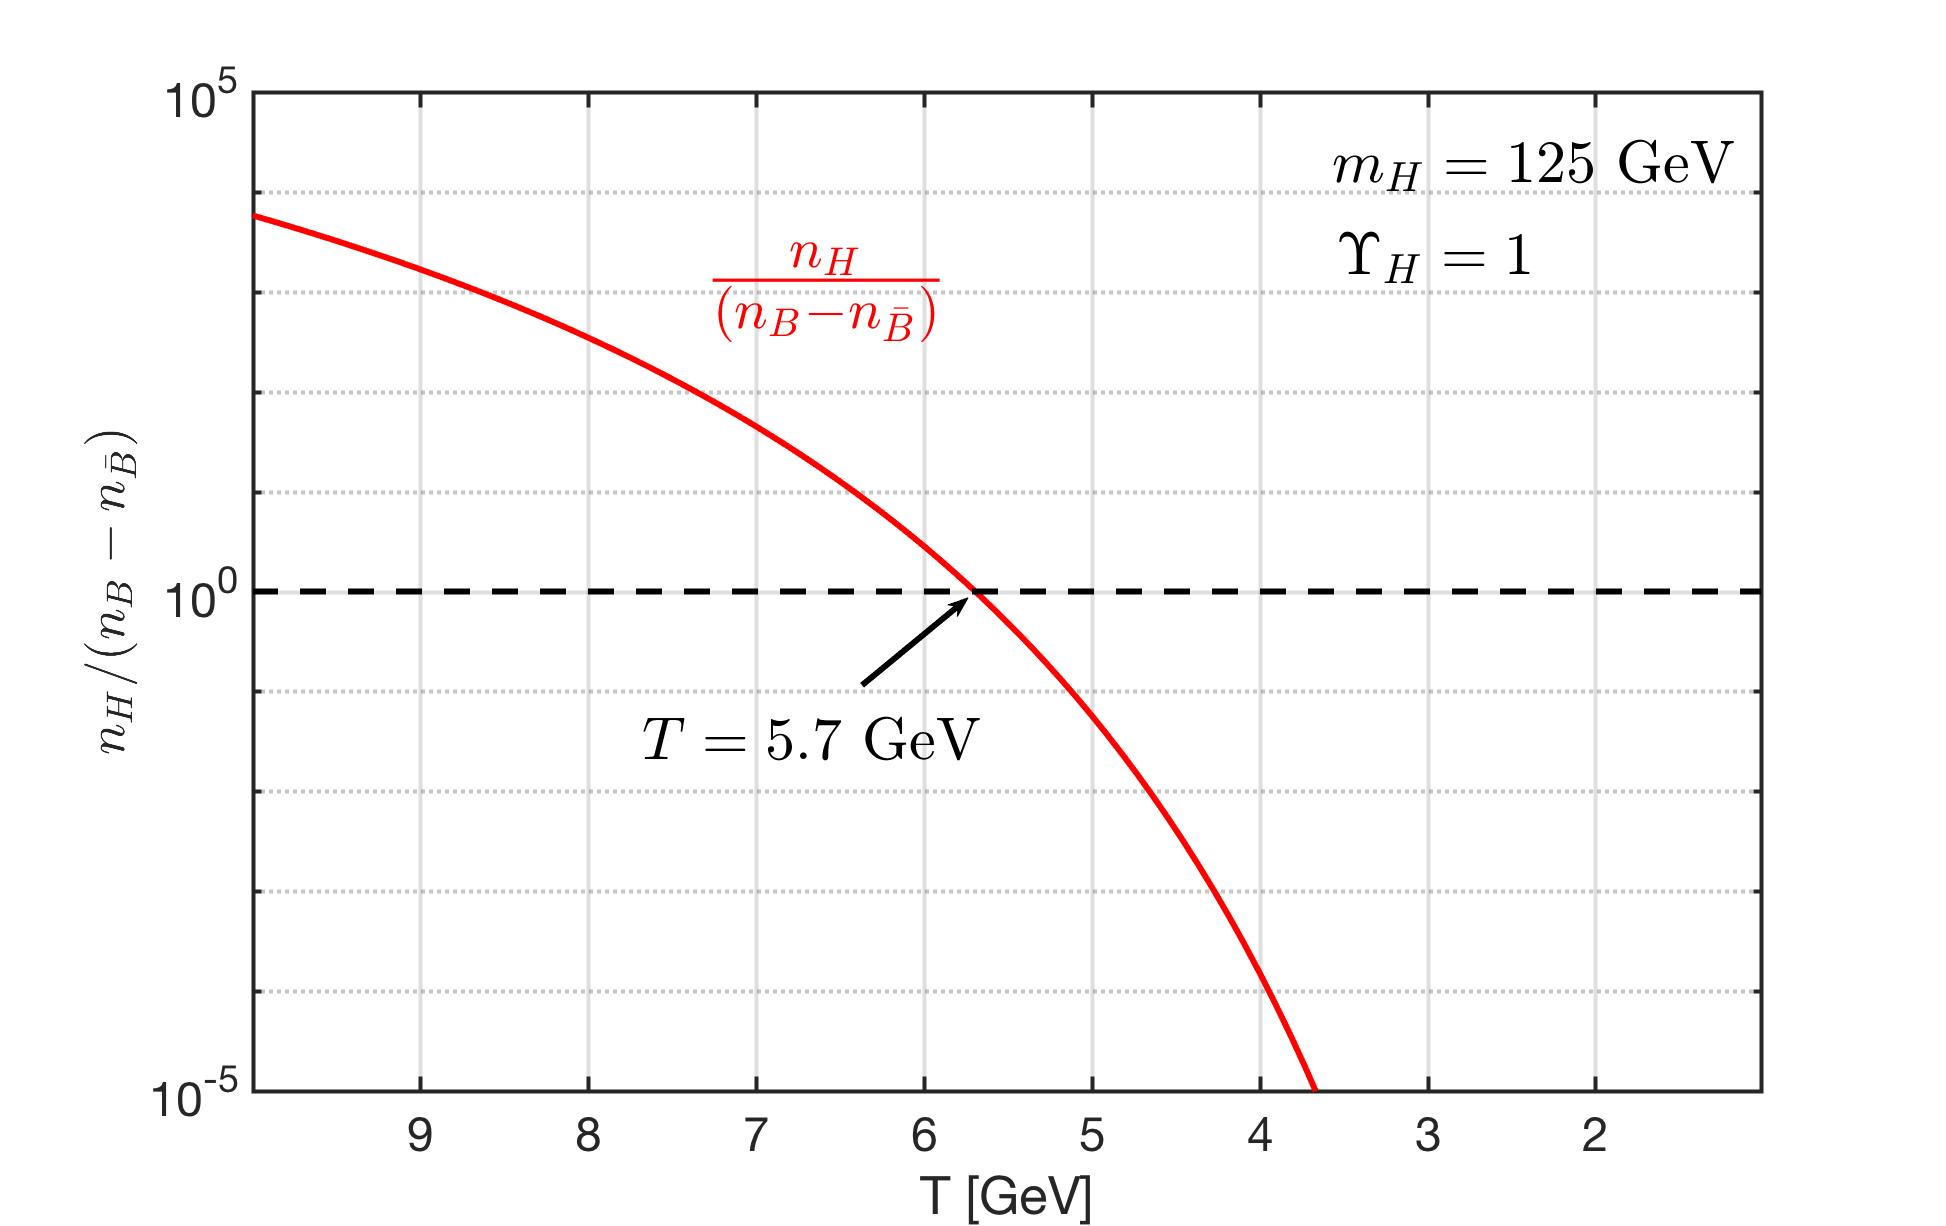
\includegraphics[width=0.9\linewidth]{./plots/HiggsDensityRatio}}
\centerline{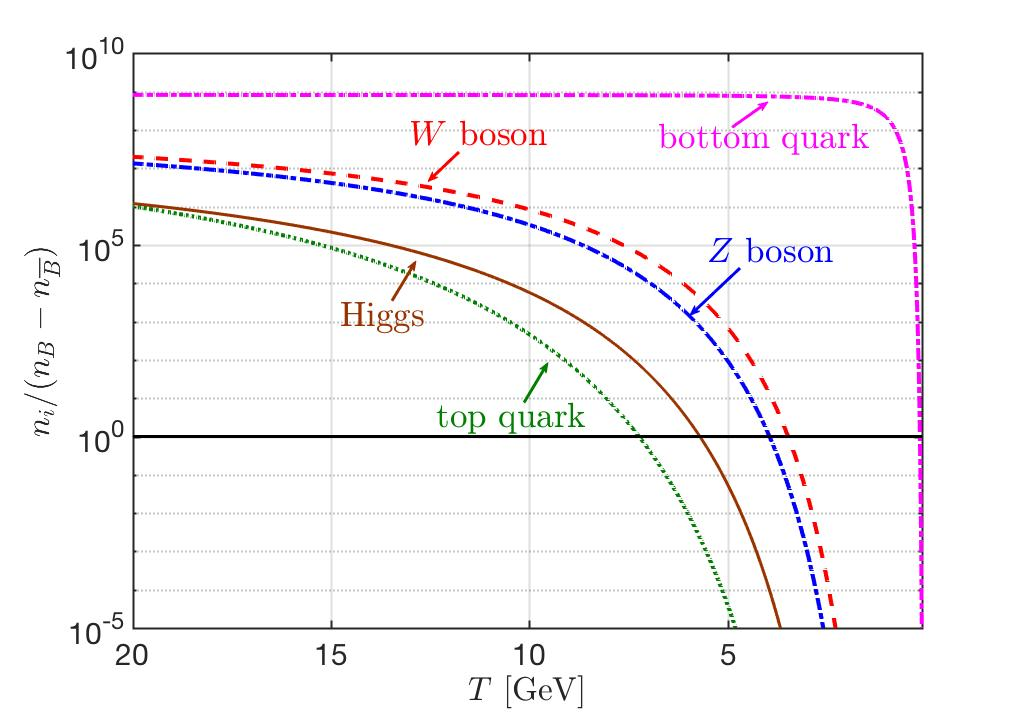
\includegraphics[width=0.85\linewidth]{./plots/ni_over_nb_vs_T-new.jpg}}
\caption{{\color{black} The ratio between thermal equilibrium density of heavy particles $t,h, \mathrm{Z,W}, b$ with the baryon excess density $n_B-n_{\bar B}$ as a function of temperature $20\GeV>T>0.1\GeV$. \radapt{Yang:2024ret}
}}
\label{HiggsDensity:fig} 
\end{figure}
%%%%%%%%%%%%%%%%%%%%%%%%%%%%%%%%%%%%%%%%%%%%%%%%%%%%%%%%%%%%%%%%%%%

{\color{black}Aside of the Higgs-particle we also see in \rf{HiggsDensity:fig} all other heavy particle thermal abundances normalized to baryon excess: the top quark with $m_t=172.7\GeV$ (dotted green), gauge bosons $m_\mathrm{W}=80.4\GeV$ (dashed red), and $m_\mathrm{Z}=91.19\GeV$ (dot-dashed blue). The relatively light $m_b=4.18\GeV$ bottom quark (dashed-dotted violet) reaches relatively quickly the asymptotic value of the ratio, $10^{9}$. We see that the these respective relative ratios reach unity $n_i/(n_B-n_{\bar{B}})\to 1$ at temperatures: $T_t=7.0$\,GeV , $T_h=5.7$ GeV, $T_\mathrm{Z}=3.9$\,GeV, $T_\mathrm{W}=3.3$\,GeV. The bottom quark remains of interest down to hadronization temperature $T_b\simeq 0.15$\,GeV. We will look at the bottom quark freeze-out in more detail below.}

%%%%%%%%%%%%%%%%%%%%%%%%%%%%
\para{Baryon asymmetry and Sakhraov conditions}
The small value of the baryon asymmetry\index{Sakharov conditions!baryogenesis} in the Universe could be interpreted as being due to the initial conditions in the Universe. However, in the current standard cosmological model, it is believed that the inflation event can erase any pre-existing asymmetry between baryons and antibaryons. In this case, we need a dynamic baryogenesis process to generate excess of baryon number compared to antibaryon number in order to create the observed baryon number today.

The precise epoch responsible for the observed matter genesis $\eta_\gamma$ in the primordial Universe has not been established yet. Several mechanisms have been proposed to explain baryogenesis with investigations typically focusing on the temperature range between GUT (grand unified theory) phase transition $T_\mathrm{G}\simeq10^{16}\,\mathrm{GeV}$ and the EW phase transition near $T_\mathrm{W}\simeq130\,\mathrm{GeV}$ \cite{Kuzmin:1985mm,Kuzmin:1987wn,Arnold:1987mh,Kolb:1996jt,Riotto:1999yt,Nielsen:2001fy,Giudice:2003jh,Davidson:2008bu,Morrissey:2012db,Canetti:2012zc}. {\color{black}The EW phase transition temperature regime was favored before mass of the Higgs-particle became known to be too heavy to allow a strong EW phase transition.}

In 1967, Andrei Sakharov formulated the three conditions necessary to permit baryogenesis in the primordial Universe~\cite{Sakharov:1967dj} and in 1988 he refined the three conditions as follows~\cite{Sakharov:1988vdp}:
\begin{subequations}\label{Sakharov}
\begin{align}
 &\text{Absence of baryonic charge conservation}\\
 &\text{Violation of CP-invariance}\index{CP
 violation}\\
&\text{Non-stationary conditions in absence of local thermodynamic equilibrium}
\end{align}
\end{subequations}
{\color{black} In the following we discuss these three Sakharov conditions for matter asymmetry to form, and argue that these conditions  could be satisfied during the entire cosmic QGP era. We will study below in more detail the bottom quark case and argue for the Higgs-particle case. Other cases are possible. We begin our considerations with the second and third condition in \req{Sakharov} above as these can easily be recognized in laboratory and/or theoretical studies of the cosmic plasma dynamics. We discuss the first condition last.}

The second Sakharov \req{Sakharov} condition requiring $CP$ (charge conjugation $\times$ parity)  violation assures us that we can recognize, in universal manner, the difference between matter and antimatter. Clearly, we could not enhance one form with reference to the other without being able to tell matter from antimatter. $CP$ violation allows us to share with another distant civilization that we are made of matter. A nice textbook discussion showing how to do this using the Kaon system CP violation is offered by Perkins~\cite{Perkins:1982xb}.

The third Sakharov condition \req{Sakharov} is a requirement for departure from thermal equilibrium which allows the breaking of detailed balance\index{detailed balance} condition: It is evident that in thermal equilibrium, the net effect of baryogenesis processes is cancelled out by equality between the  forward and back-reactions. {\color{black}Breaking of detailed balance must be non-stationary in the sense that it does not disappear entirely slowing down the Universe expansion $H\to 0$. In other words for baryogenesis to work the breaking of detailed balance must rely on the competition between microscopic processes, and not on a competition of microscopic processes with the Hubble parameter appearing in the Einstein-Vlasov equation \req{Hubble:Boltzmann}. We fully agree here with Sakharov's more precise thinking presented in 1988 \cite{Sakharov:1988vdp}.} 

{\color{black}Space-time domains near to phase transitions harbor non-stationary nonequilibrium in the expanding Universe. However, proximity of phase transformation invoked usually is not an exclusive physical environment. We will demonstrate within PP-SM how another opportunity in the primordial plasma arises: A competition between strong and EW interaction. Strong interactions can be rendered relatively weak due to mass thresholds.} 

We distinguish kinetic (momentum distribution) and chemical (particle abundance) equilibrium. This is so since kinetic equilibrium\index{kinetic equilibrium} is usually established much more quickly, while abundance yields are more difficult to establish, especially so for particles with masses in excess, or at least similar to ambient temperatures~\cite{Koch:1986ud,Birrell:2014gea}. {\color{black}This distinction allows to recognize that detailed balance can arise without a strict chemical equilibrium condition. This is seen in other cosmic and astrophysical environments, including the nucleosynthesis processes in the Universe (BBN) and stars.}  

Specifically for all heavy primordial particles including the top $t$ and bottom $b$ quarks, W and Z gauge bosons, and the Higgs-particle $h$, we observe that when the Universe expands and temperature cools down well below the particle mass, the production process and decay processes create a stationary equilibrium with detailed balance outside of equilibrium. Higgs-particle is an excellent candidate for non-stationary effects due to its small and even vanishing coupling to the massless and low mass particle plasma. 

We believe that the presence of chemical (abundance) nonequilibrium
{\color{black}is a required but not sufficient condition for a baryogenesis environment. We need further either time dependence of chemical non-equilibrium processes or a sufficiently weak coupling of one of the involved particles to the thermal background in order to extend the potential for baryogenesis to a much wider temperature domain, beyond the proximity of the EW phase transition condition. Study of the Higgs-particle in this context is one of our ongoing research challenges. However, in this work
}
we use the case of bottom quarks to demonstrate the mechanism we are exploring. We interpret the third condition of Sakharov in our specific context as follows:
\begin{itemize}
\item Non-stationary conditions in absence of local thermodynamic equilibrium $\Longrightarrow$ Absence of detailed balance associated with nonequilibrium yields and non-stationary particle abundance evolution.
\end{itemize} 

{\color{black} We now return to consider the first Sakharov condition \req{Sakharov}.  So far all efforts to create consistent description of baryogenesis based on well studied EW phase transition near $T=130$\,GeV has not been able to generate the observed baryon asymmetry \cite{Kuzmin:1985mm,Kuzmin:1987wn,Arnold:1987mh,Kolb:1996jt,Riotto:1999yt,Nielsen:2001fy,Giudice:2003jh,Davidson:2008bu,Morrissey:2012db,Canetti:2012zc}. An ad-hoc `far'-primordial to the era of EW  phase transition baryon-antibaryon asymmetry creation seems less `attractive', in the sense that we push back baryogenesis to an unknown cosmic era with mechanisms well beyond the scope of known PP-SM. Even so this is the conclusion reached after several decades of study of the EW-baryogenesis. We refer to excellent review of this efforts was presented by Morrissey and Ramsey-Musolf \cite{Morrissey:2012db} which work invites new baryogenesis physics before EW phase transition, and to Canetti, Drewes,  and Shaposhnikov \cite{Canetti:2012zc}. We defer to these reviews in regard to intricate details of EW-baryogenesis  addressed in depth there: Within the PP-SM the sphaleron mechanism plays the pivotal role (see also \url{https://en.wikipedia.org/wiki/Sphaleron} sourced September 2024) both in erasing any baryon asymmetry in presence of 2nd order EW phase transition and in creating assymetry in presence of 1st order transition. The EW phase transition is, considering PP-SM parameters, widely accepted to be 2nd order. This has stimulated a not yet conclusive search for BSM (beyond standard model) extension allowing a 1st order EW transition while not contradicting the established PP-SM properties.}

{\color{black}However, this  widely adopted conclusion to look `beyond', either in temperature or PP-SM is not fully compelling. We believe that the observed baryon-antibaryon  asymmetry can originate in the evolution of the cosmic QGP after EW transition down to hadronization condition provided that there is a  not yet discovered direct baryon conservation violating elementary process, which, for example, protects the $B-L$ (baryon minus lepton) quantum number. This is so since PP-SM does not contain baryon or lepton conservation and several minimal extensions that have been considered conserve $B-L$.  We refer to Nath and Perez \cite{Nath:2006ut} for a wider scope review of baryon number non-conservation. }

{\color{black}We note that the experimentally known limits on baryon number violating decay of protons were obtained at zero temperature, a very different environment compared to primordial QGP. This search could be extended to study of heavy particle decays: Of interest here would be baryon conservation violating decay of heavy elementary particles ($t$, $h$, W, Z, $b$). The current experimental data lack required precision to exclude  baryon number violation at the sub-nano-level required to assure that these processes do not participate in cosmic baryogenesis.} 
 
{\color{black}Another path to recognize a mechanism of baryon excess generation is the discovery of an (effective) force in primordial QGP that could create large domain separation of baryons and antibaryons. In general the elementary quark or lepton antimatter is electrically attracted to matter. However, in the strong interaction sector there could be hidden baryon number differentiating processes:  Interlocking flavor and color organization of quark matter in the so-called CFL-phase (color-flavor locked phase) \cite{Rajagopal:2000ff,Alford:2001zr,Kaplan:2001qk} is here of interest. Another context worth further exploration  are neutral composite anti-baryonic particles (\eg\ anti-neutrons, $\overline\Lambda(uds)$ and more exotic variants) present abundantly during the mixed phase QGP hadronization process. We will not further explore this alternative which has not attracted much attention so far. }


%%%%%%%%%%%%%%%%%%%%%%%%%%%%%%%
\para{Production and decay of Higgs-particle in QGP}
The  uniqueness of the Higgs-particle\index{Higgs-particle} among heavy PP-SM particles is also due to its stability: The total width is $\Gamma_h\simeq 2.5\times\,10^{-5}m_h$. This combines with the unexpected low value of $T=5.7\GeV$ of interest where the Higgs-particle yield is equal to the baryon asymmetry in the Universe. This motivates us to examine here, in a qualitative manner, the dynamical abundance of the Higgs-particle in the QGP epoch, seeking the eventual non-stationary condition needed for baryogenesis 

The Higgs-particle predominantly decays via the $W,Z$ decay channels as follows:
\begin{align}
h\longrightarrow WW^\ast\,. ZZ^\ast\longrightarrow\mathrm{anything}\,.
\end{align}
Here $W^\ast,Z^\ast$ represent the production of virtual off-mass-shell gauge bosons decaying rapidly into relevant particle pairs. Therefore, once Higgs-particle decays via this channel, at least four particles are ultimately formed and there is no path back for $T\ll m_h$. This is so since the spectral energy of the four produced particles, on average $31\GeV$, is epithermal compared to the ambient plasma at the low temperature of interest near to $T\simeq 6\GeV$. Therefore, a back-reaction production of Higgs-particle in this channel would be weaker destroying the detailed balance required for the chemical equilibrium yield. 

In the QGP epoch, the dominant production of the Higgs-particle is the bottom quark pair fusion reaction: 
\begin{align}
b+\overline{b}\longrightarrow h\,,
\end{align}
which is the inverse to the important but by far not dominant decay process of $h\to b+\overline{b}$. This means that in first approximation the detailed balance Higgs-particle yield is reached well below the chemical equilibrium.

However, there could be considerable deviation from kinetic momentum equilibrium as well. This is so since bottom fusion will in general produce a Higgs-particle out of kinetic momentum equilibrium. A heavy particle immersed into a plasma of lighter particles requires many, many collisions to equilibrate the momentum distribution. This is a well-known kinetic theory result. Moreover, the Higgs-particle interacts weakly with all lower mass particles in QGP present at $T<10\GeV$. 

The Higgs-particle is by far the best candidate to fulfill the Sakharov non-stationary condition in the primordial Universe at a temperature range of interest to baryogenesis. A full dynamic study leading to proper understanding of the off-chemical and off-kinetic equilibrium non-stationary abundance of Higgs-particle is one of the near future projects we consider, and is therefore today beyond the scope of this report. 

%%%%%%%%%%%%%%%%%%%%%%%%%%%%%%%%
\subsection{Heavy quark production and decay}
\label{sec:heavyQ}
%%%%%%%%%%%%%%%%%%%%%%%%%%%%%%%%%
\index{quark!abundance}\index{QGP!quark abundance}
\para{Heavy quarks in the primordial QGP}
The primordial QGP refers to the state of matter that existed in the primordial Universe, specifically for time $t\approx 20\, \mathrm{\mu s}$ after the Big-Bang\index{Big-Bang}. At that time the Universe was controlled by the strongly interacting particles: quarks and gluons. In this chapter, we study the heavy bottom and charm flavor quarks near to the QGP hadronization\index{hadrons!hadronization} temperature, $0.3\,\mathrm{GeV}>T>0.15\,\mathrm{GeV}$, and examine the relaxation time for the production and decay of bottom/charm quarks. Then we show that the bottom quark nonequilibrium occur near to QGP–hadronization and creates the arrow in time in the primordial Universe.
 
In the QGP epoch, up and down $(u,d)$ (anti)quarks are effectively massless and provide, along with gluons, some leptons, and photons, the thermal bath defining the thermal temperature. Strange $(s)$ (anti)quarks are also found to be in equilibrium considering their weak, electromagnetic, and strong interactions; indeed this equilibrium continues in hadronic epoch until $T\approx13\MeV$~\cite{Yang:2021bko}. 

The massive top $(t)$ (anti)quarks couple to the plasma via the channel~\cite{ParticleDataGroup:2022pth} 
\begin{equation}
t\leftrightarrow W+b\,,\qquad \Gamma_t=1.4\pm0.2\,\mathrm{GeV}\,.
\end{equation}
As is well-known, the width prevents formation of bound toponium states. Given the large value of $\Gamma_t$ there is no freeze-out of top quarks until $W$ itself freezes out. To address the top quarks in QGP, a dynamic theory for $W$ abundance is needed, a topic we will embark on in the future. 
 
The semi-heavy bottom $(b)$ and charm $(c)$ quarks can be produced by strong interactions via quark-gluon pair fusion processes. These quarks decay via weak interaction decays and their abundance depends on the competition between the strong interaction fusion processes at low temperature inhibited by the mass threshold, and weak decay reaction rates.

In the following we consider the temperature near QGP hadronization $0.3\,\mathrm{GeV}>T>0.15\,\mathrm{GeV}$, and study the bottom and charm abundance by examining the relevant reaction rates of their production and decay.
In thermal equilibrium the number density of light quarks can be evaluated in the massless limit, and we have\index{number density of quark}
\begin{align}\label{FermiN}
n_q=\frac{g_{q}}{2\pi^2}\,T^3 F(\Upsilon_q)\;, \quad F=\int_0^\infty \frac{x^2dx}{1+\Upsilon_q^{-1}e^x}\;,
\end{align}
where $\Upsilon_q$ is the quark fugacity\index{fugacity!quark}. We have $ F(\Upsilon_q=1)=3\,\zeta(3)/2$ with the Riemann zeta function $\zeta(3)\approx1.202$.
The thermal equilibrium number density of heavy quarks with mass $m\gg T$ can be well described by the Boltzmann expansion of the Fermi distribution function, giving
\begin{align}\label{BoltzN}
n_{q}\!=\!\frac{g_{q}T^3}{2\pi^2}\sum_{n=1}^{\infty}\frac{(-1)^{n+1}\Upsilon_q^n}{n^4}\left(\frac{n\,m_{q}}{T}\right)^{\!2}\!K_2\left(\frac{n\,m_{q}}{T}\right),
\end{align} 
where $K_2$ is the modified Bessel\index{Bessel function} functions of integer order `$2$'. In the case of interest, when $m\gg T$, it suffices to consider the Boltzmann\index{Boltzmann!approximation} approximation and to keep the first term $n=1$ in the expansion. The first term $n=1$ also suffices for both charmed $c$-quarks and bottom $b$-quarks, giving
\begin{align}
&n_{b,c}={\Upsilon_{b,c}\,}n^{th}_{b,c},\qquad n^{th}_{b,c}=\frac{g_{b,c}}{2\pi^2}\,T^3\left(\frac{m_{b,c}}{T}\right)^2\,K_2(m_{b,c}/T).
\end{align}
However, for strange $s$ quarks, several terms are needed. 

In~\rf{number_entropy_b002} we show the equilibrium ($\Upsilon=1$) bottom and charm number density per entropy density ratio as a function of temperature $T$. The $b$-quark mass parameters shown are $m_b=4.2\,\mathrm{GeV}$ (blue) dotted line, $m_b=4.7\,\mathrm{GeV}$ (black) solid line, and $m_b=5.2\,\mathrm{GeV}$ (red) dashed line. For $c$-quark, $m_c=0.93\,\mathrm{GeV}$ (blue) dotted line, $m_c=1.04\,\mathrm{GeV}$ (black) solid line, and $m_c=1.15\,\mathrm{GeV}$ (red) dashed line. The entropy density\index{entropy!density} is given by~\req{entropy} and only light particles contribute significantly. Thus the result we consider is independent of the actual abundance of $c$, $b$ and other heavy particles. 

%%%%%%%%%%%%%%%%%%%%%%%%%%%%%%%%%%%%%%%
\begin{figure}
\centerline{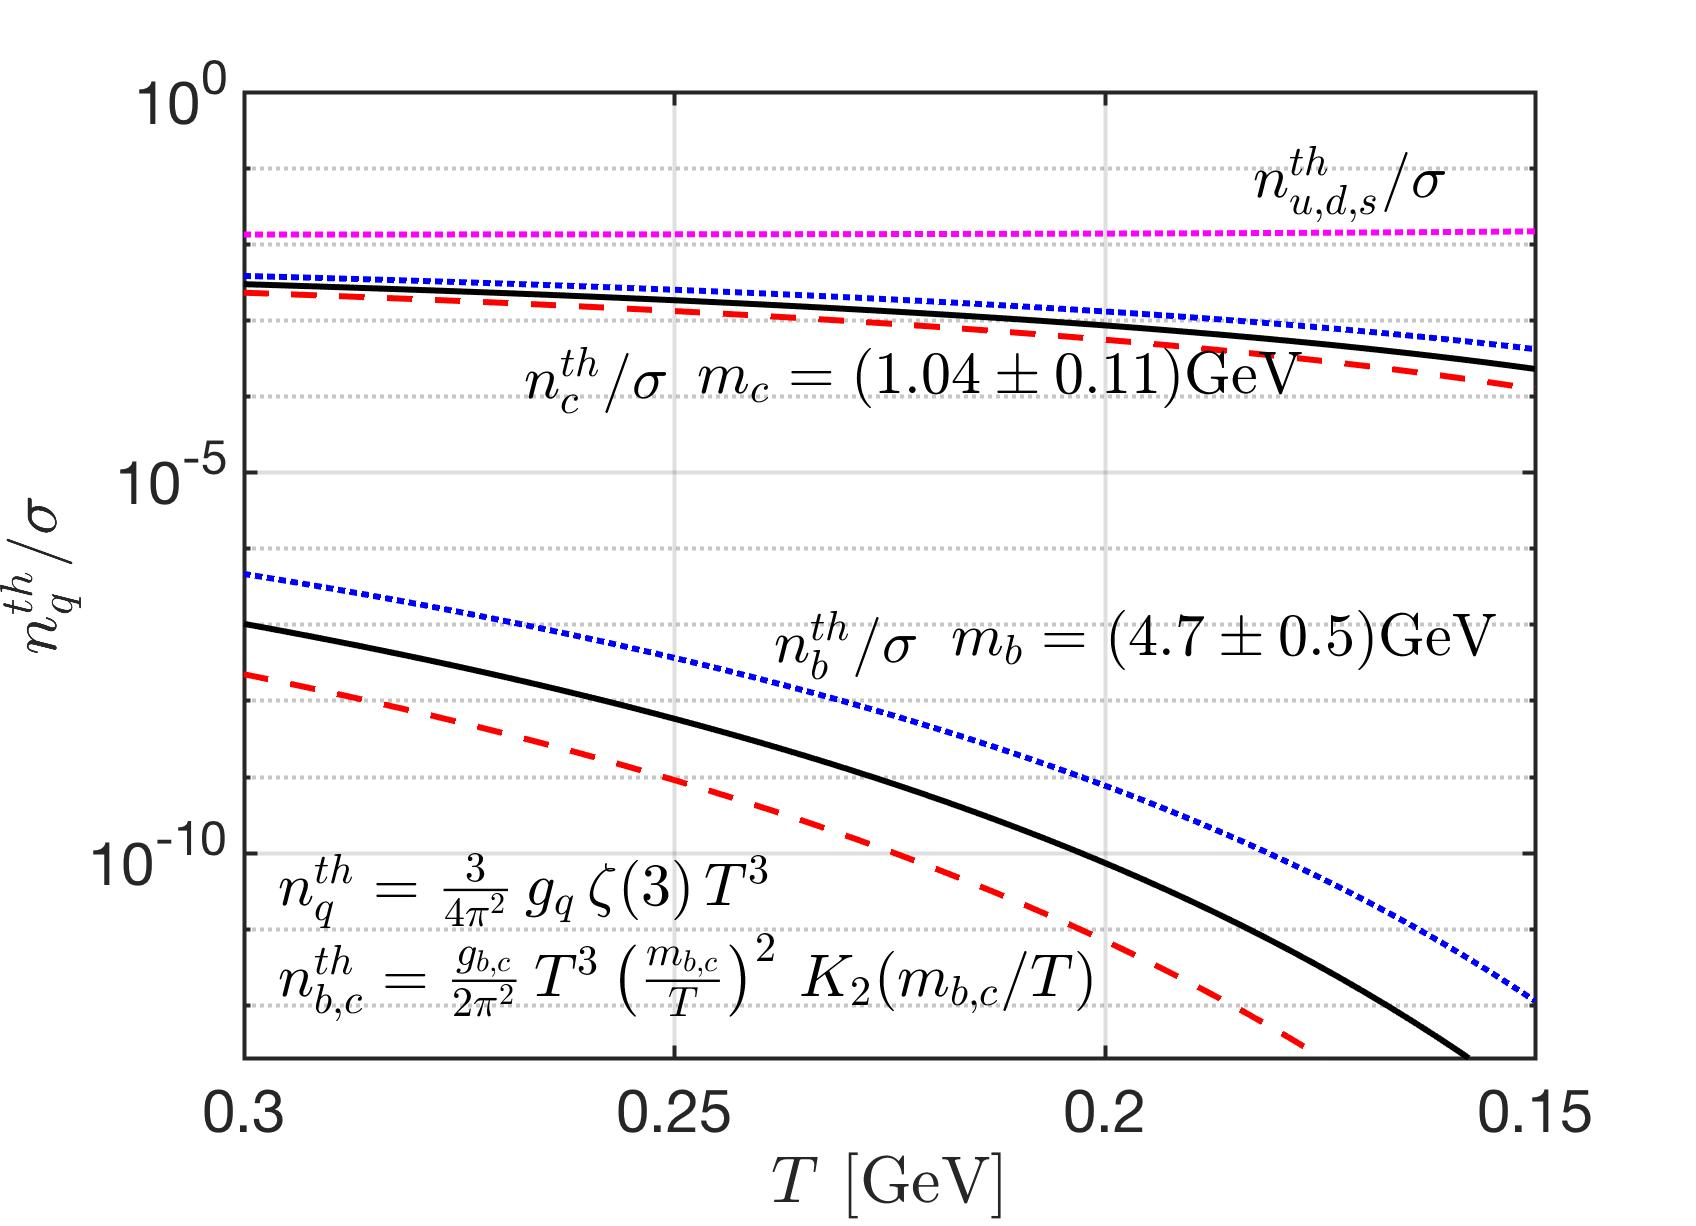
\includegraphics[width=0.8\linewidth]{./plots/bcQuarkDensity_new}}
\caption{
The equilibrium charm and bottom quark number density normalized by entropy density, as a function of temperature in the primordial Universe, see text for discussion of different mass values. \radapt{Yang:2024ret}}
\label{number_entropy_b002} 
\end{figure}
%%%%%%%%%%%%%%%%%%%%%%%%%%%%%%%%%%%%%%%%%%% 

The $m_b\simeq 5.2\,\mathrm{GeV}$ is a typical potential model mass used in modeling bound states of bottom, and $m_b=4.2,\,4.7\,\mathrm{GeV}$ is the current quark mass at low and high energy scales. In~\rf{number_entropy_b002} we see that the charm abundance in the domain of interest $0.3\,\mathrm{GeV}>T>0.15\,\mathrm{GeV}$ is about $10^4\sim 10^{9}$ times greater than the abundance of bottom quarks. This implies that the small $b$,$\bar b$ quark abundance is embedded in a large background comprising all lighter $u,d,s,c$ quarks and anti-quarks, as well as gluons $g$.

In the following we will calculate the production and decay rate for bottom and charm quarks and compare to the Universe expansion rate. We will show that in the epoch of interest to us the characteristic Universe expansion time $1/H$ is much longer than the lifespan and production time of the bottom/charm quark. In this case, the dilution of bottom/charm quark due to the Universe expansion is slow compare to the the strong interaction production, and the weak interaction decay of the bottom/charm. Any abundance nonequilibrium will therefore be nearly stationary. 

It is important for following analysis to know that the expansion of the Universe is the slowest process, allowing many microscopic reactions at a `fixed' temperature range $T$ to proceed. To show this we evaluate the Hubble\index{Hubble!parameter} relation to obtain $1/H$\,[s]
\begin{align}
H^2=\frac{8\pi G_N}{3}\left(\rho_\gamma+\rho_{\mathrm{lepton}}+\rho_{\mathrm{quark}}+\rho_{g,{W^\pm},{Z^0}}\right)
\,.
\end{align}
The effectively massless particles and radiation dominate particle energy density $\rho_i$, defining the speed of expansion of the Universe within temperature range $130\, \mathrm{GeV}>T>0.15\,\mathrm{GeV}$. We have the following particles: photons, $8$ color charge gluons, $W^\pm$, $Z^0$, three generations of $3$ color charge quarks and leptons in the primordial QGP. The characteristic Universe expansion time constant $1/H$ is seen in~\rf{BCreaction:fig} below. In the epoch of interest to us $0.3\,\mathrm{GeV}>T>0.15\,\mathrm{GeV}$, the Hubble time $1/H\approx10^{-5}\,\mathrm{s}$, which is much longer than the microscopic lifespan and production time of the bottom and charm quarks we study 

%%%%%%%%%%%%%%%%%%%%%%%%%%%%%%%%%%%%%
\para{Quark production rate via strong interaction}
In primordial QGP\index{quark!production rate}, the bottom and charm quarks can be produced from strong interactions via quark-gluon pair fusion processes. For production, we have the following processes
\begin{align}
 q+\bar{q}&\longrightarrow b+\bar b,\qquad q+\bar{q}\longrightarrow c+\bar c,\\
 g+g&\longrightarrow b+\bar b,\qquad g+g\longrightarrow c+\bar c\,.
\end{align}

For the quark-gluon pair fusion processes\index{bottom quark!production rate}
%\begin{align}
% q+q&\longrightarrow b+\bar b,\qquad q+q\longrightarrow c+\bar c,\\
% g+g&\longrightarrow b+\bar b,\qquad g+g\longrightarrow c+\bar c,
%\end{align}
the evaluation of the lowest-order Feynman diagrams yields the cross-sections~\cite{Letessier:2002ony}:
\begin{align}
&\sigma_{q\bar{q}\rightarrow b\bar{b},c\bar{c}}=\frac{8\pi\alpha_s^2}{27s}\left(1+\frac{2m_{b,c}^2}{s}\right)w(s),\,\qquad w(s)=\sqrt{1-{4m^2_{b,c}}/{s}},\\
&\sigma_{gg\rightarrow b\bar{b},c\bar{c}}=\!\frac{\pi\alpha_s^2}{3s}\bigg[\left(1\!+\!\frac{4m^2_{b,c}}{s}\!+\!\frac{m^4_{b,c}}{s^2}\right)\ln{\left(\frac{1+w(s)}{1-w(s)}\right)}\!-\!\left(\frac{7}{4}\!+\!\frac{31m^2_{b,c}}{4s}\right)w(s)\bigg],
\end{align} 
where $m_{b,c}$ represents the mass of bottom or charm quark, $s$ is the Mandelstam variable, and $\alpha_s$ is the QCD coupling constant. Considering the perturbation expansion of the coupling constant $\alpha_s$ for the two-loop approximation~\cite{Letessier:2002ony}, we have:
\begin{align}
\alpha_s(\mu^2)=\frac{4\pi}{\beta_0\ln({\mu^2/\Lambda^2})}\bigg[1-\frac{\beta_1}{\beta_0}\frac{\ln(\ln{(\mu^2/\Lambda^2)})}{\ln(\mu^2/\Lambda^2)}\bigg],
\end{align}
where $\mu$ is the renormalization energy scale and $\Lambda^2$ is a parameter that determines the strength of the interaction at a given energy scale in QCD. The energy scale we consider is based on required gluon/quark collisions above $b\bar b$ energy threshold, so we have $\mu=2m_b+T$. For the energy scale $\mu>2m_b$ we have $\Lambda=180\sim230\MeV$ ($\Lambda\approx205\MeV$ in our calculation), and the parameters $\beta_0=11-2n_f/3$, $\beta_1=102-38n_f/3$ with the number of active fermions $n_f=4$. 

%%%%%%%%%%%%%%%%%%%%%%%%%%%%%%%%%%%%%%%
\begin{figure} 
\centerline{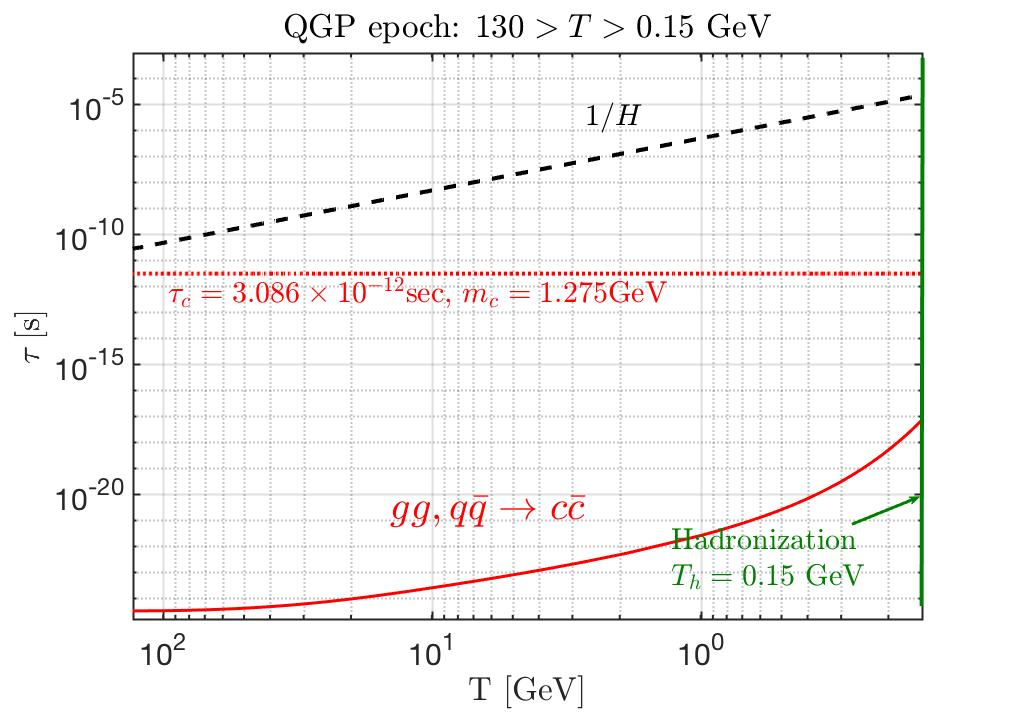
\includegraphics[width=0.49\linewidth]{./plots/CharmQuark_QGP.jpg}
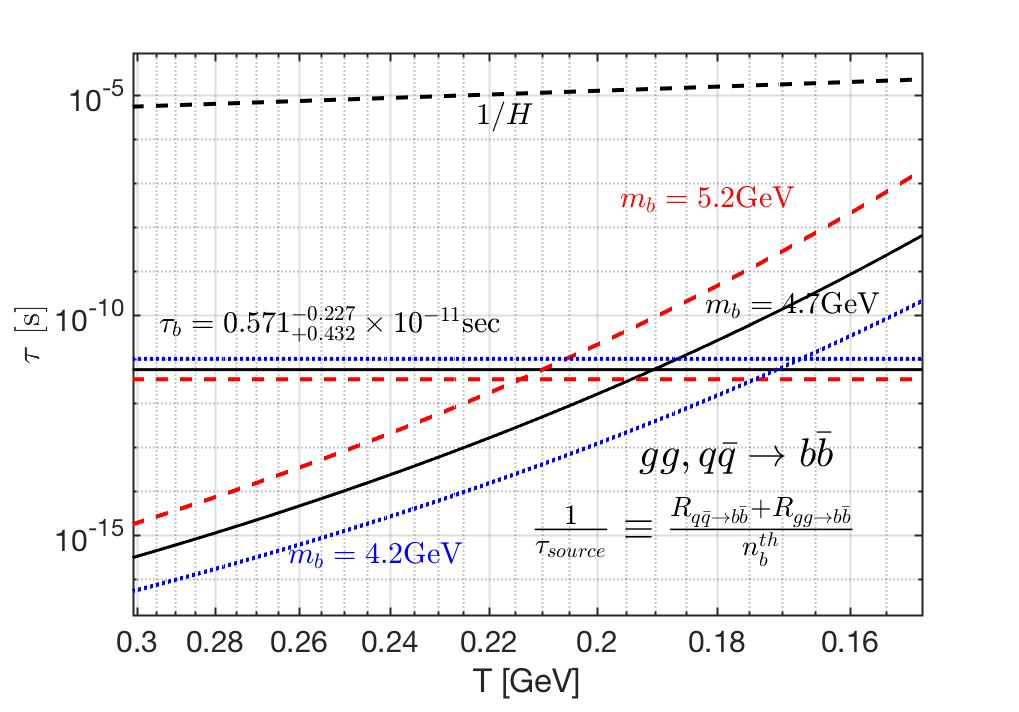
\includegraphics[width=0.49\linewidth]{./plots/BQuarkReactionTime_bottom.jpg}}
\caption{Comparison of Hubble\index{Hubble!time} time $1/H$, quark lifespan $\tau_{q}$, and characteristic time for production via quark, gluon pair fusion. The upper frame for charm $c$-quark in the entire QGP epoch $T$ rang; the lower frame for bottom $b$-quark amplifying the dynamic detail balance $T\simeq 200\MeV$. Both figures end at the hadronization temperature of $T_{H}\approx150\MeV$. See text for additional information. \cccite{Rafelski:2023emw}. \radapt{Yang:2024ret}}
\label{BCreaction:fig}
\end{figure}
%%%%%%%%%%%%%%%%%%%%%%%%%%%%%%%%%%%%%%%

In general the thermal reaction rate per unit time and volume $R$ can be written in terms of the scattering cross-section as follows~\cite{Letessier:2002ony}:
\begin{align}
R\equiv\sum_i\int_{s_{th}}^\infty\!ds\,\frac{dR_i}{ds}=\sum_i\int_{s_{th}}^\infty\!ds\,\sigma_i(s)\,P_i(s),
\end{align}
where $\sigma_i(s)$ is the cross-section of the reaction channel $i$, and $P_i(s)$ is the number of collisions per unit time and volume. Considering the quantum nature of the colliding particles (i.e., Fermi and Bose distribution)\index{Bose!distribution}\index{Fermi!distribution} with the massless limit and chemical equilibrium\index{chemical equilibrium} condition ($\Upsilon=1$), we obtain~\cite{Letessier:2002ony}
\begin{align}
&P_i(s)=\frac{g_1g_2}{32\pi^4}\,\frac{T}{1+I_{12}}\frac{\lambda_2}{\sqrt{s}}\!\sum_{l,n=1}^{\infty}\!(\pm)^{l+n}\frac{K_1(\sqrt{lns}/T)}{\sqrt{ln}},\\
&\lambda_2\equiv\left[s-\left(m_1+m_2\right)^2\right]\,\left[s-\left(m_1-m_2\right)^2\right],
\end{align}
where $+$ is for boson and $-$ is for fermions, and the factor $1/(1+I_{12})$ is introduced to avoid double counting of indistinguishable pairs of particles. $I_{12}=1$ for identical pair of particles, otherwise $I_{12}=0$. Hence the total thermal reaction rate per volume for bottom quark production can be written as
\begin{align}
\label{Bquark_Source}
R^{\mathrm{Source}}_{b,c}=\int^\infty_{s_{th}}ds\,\bigg[\sigma_{q\bar{q}\rightarrow b\bar{b},c\bar{c}}\,P_q+\sigma_{gg\rightarrow b\bar{b},c\bar{c}}\,P_g\bigg]
%=R_{q\bar{q}\rightarrow b\bar{b},c\bar{c}}+R_{gg\rightarrow b\bar{b},c\bar{c}}
\,.
\end{align}
We introduce the bottom/charm quark relaxation time for the quark-gluon pair fusion as follows:
\begin{align}
\label{relaxation_time}
&{\tau_{b,c}^{\mathrm{Source}}}\equiv\frac{dn_{b,c}/d\Upsilon_{b,c}}{R^{\mathrm{Source}}_{b,c}}\;,
\end{align}
where $dn_{b,c}/d\Upsilon_{b,c}=n^{th}_{b,c}$ in the Boltzmann\index{Boltzmann!approximation} approximation. The relaxation time is on the order of magnitude of time needed to reach chemical equilibrium. 

In~\rf{BCreaction:fig} we show the characteristic time for $b$ and $c$ quark strong interaction production. The $c$ quark (upper frame) is shown in the entire QGP temperature range. We note the vast 15 orders of magnitude difference between the Hubble time and the rate of production. This means there will be very many microscopic cycles of charm production decay, erasing any non-stationary effect. For $b$ (lower frame) we restrict the view to temperature range in the domain of interest, $ 0.3\,\mathrm{GeV}>T> 0.15\,\mathrm{GeV}$. Three different masses $m_{b}=4.2\GeV$ (blue short dashes), $4.7\GeV$, (solid black), $5.2\GeV$ (red long dashes) for bottom quarks are shown. 
 
%%%%%%%%%%%%%%%%%%%%%%%%%%%%%%%%
\para{Quark decay rate via weak interaction}
The bottom/charm quark decay\index{quark!weak decay rate} via the weak interaction \index{bottom quark!decay rate} 
\begin{align}
 &b\longrightarrow c+l+\overline{\nu_l}, \qquad b\longrightarrow c+q+\bar{q},\\
&c\longrightarrow s+l+\overline{\nu_l},\qquad c\longrightarrow s+q+\bar{q}\,.
\end{align}
The vacuum decay rate for $1\to2+3+4$ in vacuum can be evaluated via the weak interaction:
\begin{align}
\frac{1}{\tau_1}=&\frac{64G^2_F\,V^2_{12}\,V^2_{34}}{(4\pi)^3g_1}\,m^5_1\times\left[\frac{1}{2}{\left(1-\frac{m^2_2}{m^2_1}-\frac{m^2_3}{m^2_1}+\frac{m^2_4}{m^2_1}\right)}\mathcal{J}_1-\frac{2}{3}\mathcal{J}_2\right],
\end{align}
where the Fermi constant is $G_F=1.166\times10^{-5}\,\mathrm{GeV}^{-2}$, $V_{ij}$ is the element of the Cabibbo-Kobayashi-Maskawa (CKM) matrix~\cite{Czarnecki:2004cw}\index{CKM matrix} for quark channel and $V_{l\nu_l}=1$ for lepton channel. The functions $\mathcal{J}_1$, and $\mathcal{J}_2$ are given by
\begin{align}
&\mathcal{J}_1\!=\!\!\!\int_0^{(1-m^2_2/m^2_1)/2}\!\!\!\!\!\!\!\!dx\left(1\!-\!2x\!-\!\frac{m^2_2}{m_1^2}\right)^{\!\!2}\left[\frac{1}{(1-2x)^2}-1\right]\,,\\
&\mathcal{J}_2\!=\!\!\!\int_0^{(1-m^2_2/m^2_1)/2}\!\!\!\!\!\!\!\!dx\left(1\!-\!2x\!-\!\frac{m^2_2}{m_1^2}\right)^{\!\!3}\left[\frac{1}{(1-2x)^3}-1\right]
\,.
\end{align}
The modification due to the heat bath (plasma) is small because the bottom and charm mass $m_{b,c}\gg T$~\cite{Kuznetsova:2008jt}. In the temperature range we are interested in, the decay rate in the vacuum is a good approximation for our calculation. 

We show the lifespan for bottom and charm quarks in~\rf{BCreaction:fig}. For charm (upper frame) the decay is always much slower compared to production. This assures that the strong interaction processes can easily maintain equilibrium. Thus, during the entire era of QGP, charm quarks can be assumed to be in an equilibrium condition. 

After hadronization\index{hadrons!hadronization}, charm quarks form heavy mesons that decay into several hadronic particles. The daughter particles from charm meson decay can interact and re-equilibrate within the hadron plasma. There are very many branching reactions and some involve production of only light particles. In this case the energy required to drive the inverse reaction to produce heavy charm mesons is difficult to overcome. We believe this is causing the charm quark to vanish from the inventory shortly after hadronization, but a detailed study has not been carried out due to complexity of the situation. 

Looking at the lower frame in~\rf{BCreaction:fig}, we see that in the case of bottom quarks the decay crosses the production rate, and this happens within QGP near to $T=200\MeV$. The intersection implies that the bottom quark\index{bottom quark} freeze-out from the primordial plasma before hadronization as the production process slows down at low temperatures and the subsequent weak interaction decay leads to a dilution of the bottom quark content within the QGP plasma. All of this occurs with rates significantly faster than Hubble expansion and thus, as the Universe expands, the system departs from chemical equilibrium in near stationary manner, because of the competition between decay and production reactions in QGP. We will show how the dynamic equation cause the distribution to deviate from equilibrium with $\Upsilon\neq1$ in the temperature range below the crossing point but before the hadronization. 

%%%%%%%%%%%%%%%%%%%%%%%%%%%%
\subsection{Is baryogenesis possible in QGP phase?}\label{Bottom}
%%%%%%%%%%%%%%%%%%%%%%%%%%%%%%%%%%%%%%%%%%%%
\index{quark!bottom nonequilibrium}
\para{Bottom quark abundance nonequilibrium}
The competition between weak interaction decay and strong interaction production rates can lead to a nonequilibrium dynamic heavy quark abundance. We explore as example the case of bottom quarks in QGP. Similar considerations apply to all heavier PP-SM particles including in particular Higgs, W,Z gauge bosons, top $t$ quark. However, the case of $b$-quarks attracted our attention early on in context of baryogenesis since there is strong known CP violation\index{CP violation} also present.
 
The dynamic equation for bottom quark abundance in QGP can be written as \index{bottom quark!population equation}
\begin{align}
\label{Bquark_eq}
\frac{1}{V}\frac{dN_b}{dt}=\big(\,1-\Upsilon^2_{b}\,\big)\,R^{\mathrm{Source}}_{b}-\Upsilon_b\,R^{\mathrm{Decay}}_{b}\;,
\end{align}
where $R^{\mathrm{Source}}_{b}$ and $R^{\mathrm{Decay}}_{b}$ are the thermal reaction rates per volume of production and decay of bottom quark, respectively. The bottom source rates are the gluon and quark fusion rates \req{Bquark_Source}. The decay rate depends on whether the bottom quarks are freely present in the plasma or are bounded within mesons. We consider two extreme scenarios for the bottom quark population: 1.) all bottom flavor is free, and 2.) all bottom flavor is bounded into mesons in QGP. In~\rf{ReactionTime} we show the characteristic interaction times relevant to the abundance of bottom quarks, as well as the Hubble time $1/H$ for the temperature range of interest, $0.3\,\mathrm{GeV}> T> 0.15\,\mathrm{GeV}$.

%%%%%%%%%%%%%%%%%%%%%%%%%%%%%%%%%%%%%%
\begin{figure} 
\centerline{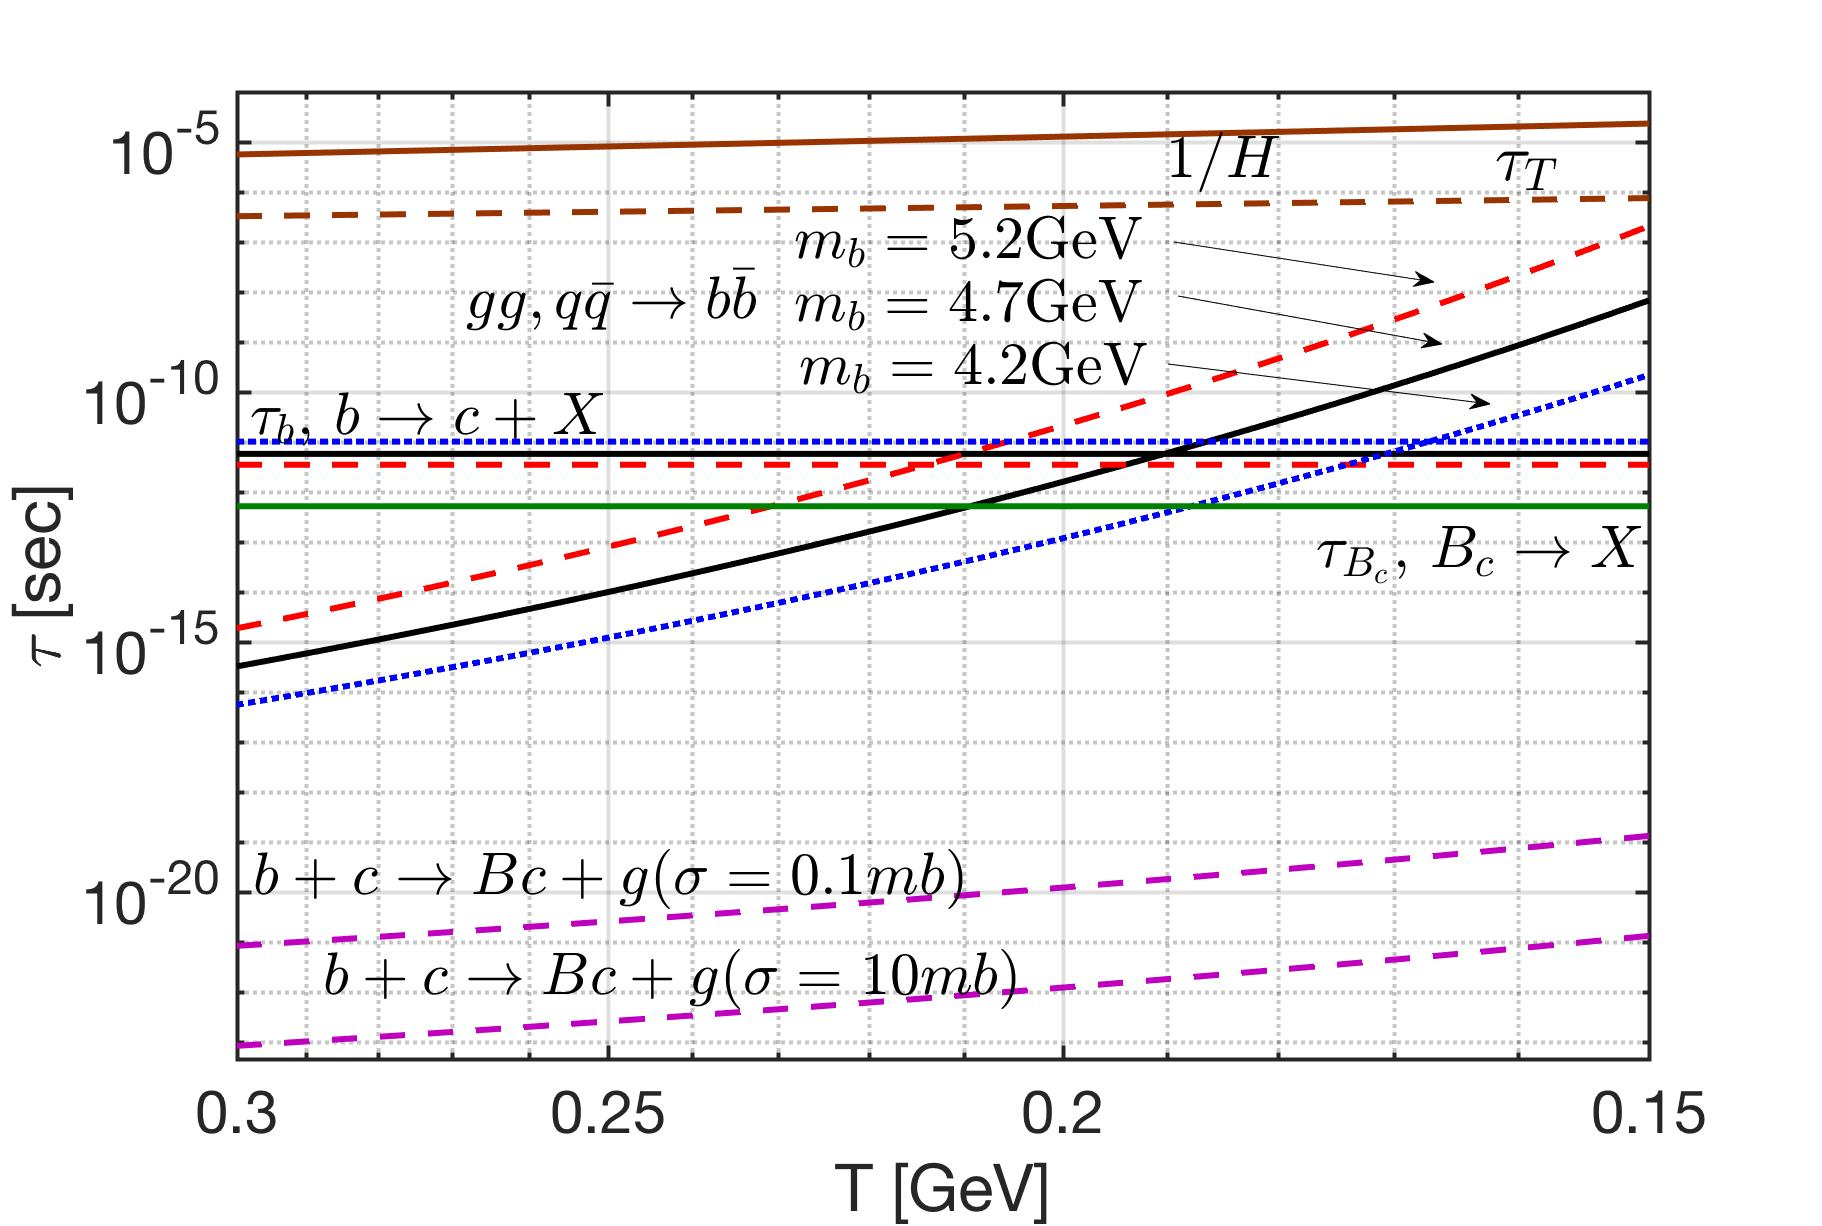
\includegraphics[width=0.85\linewidth]{./plots/BQuarkReactionTime003}}
\caption{{\color{black}Top of figure: solid (brown) line is the characteristic $1/H$[s] cosmological time as a function of temperature $0.3\,\mathrm{GeV}>T> 0.15\MeV$. Just below it dashed (braun) dilution time $\tau_T$, \req{eq:tauT}. The total strong interaction bottom production $g+g\to b+\bar{b},$, $q+\bar q\to b+\bar{b}$ relaxation time is shown for three different bottom masses: $m_b=4.2\,\mathrm{GeV}$ (blue dotted line), $m_b=4.7\,\mathrm{GeV}$ (black solid line), $m_b=5.2\,\mathrm{GeV}$ (red dashed line). The nearly horizontal lines are bottom-quark (in QGP) EW decay lifetimes $\tau_b$ with the same color coding as the production processes. Horizontal solid (green) line is the vacuum lifespan $\tau_{B_c}$. At the bottom of the figure dashed lines (purple) are in QGP plasma pre-formation process $b+c\rightarrow \mathrm{B}_c+g$ with cross-section bracketing range $\sigma=\{0.1,10\} \,\mathrm{mb}$. \radapt{Yang:2024ret}.
}}
\label{ReactionTime}
\end{figure}
%%%%%%%%%%%%%%%%%%%%%%%%%%%%%%%%%

Considering all bottom flavor is free in QGP, the bottom decay rate per volume is the bottom lifespan weighted with density of particles \req{BoltzN}, see Ref.\,\cite{Kuznetsova:2008jt}. We have
\begin{align}\hspace{0.5cm}
R^{\mathrm{Decay}}_b=\frac{dn_b/d\Upsilon_b}{\tau_b},\,\,\,\,\, \tau_b\approx0.57\times10^{-11} \mathrm{s}.
\end{align}
On the other hand, $b$,\,$\bar b$ quark abundance is embedded in a large background comprising all lighter quarks and anti-quarks (see~\rf{number_entropy_b002}). After formation the heavy $b,\,\bar b$ quark can bind with any of the available lighter quarks, with the most likely outcome being a chain of reactions 
\begin{align}
&b+q\longrightarrow\mathrm{B}+g\;,\\
&\mathrm{B}+s\longrightarrow\mathrm{B}_s+q\;,\\
&\mathrm{B}_s+c\longrightarrow\mathrm{B}_c+s\;,
\end{align}
with each step providing a gain in binding energy and reduced speed due to the diminishing abundance of heavier quarks $s, c$. To capture the lower limit of the rate of $\mathrm{B}_c$ production we show in~\rf{ReactionTime} the expected formation rate by considering the direct process $b+\overline c\rightarrow \mathrm{B}_c+g$, considering the range of cross-section $\sigma=0.1\sim10\,\mathrm{mb}$ ~\cite{Schroedter:2000ek}. The rapid formation rate of B$_c(b\bar c)$ states in primordial plasma is shown by purple dashed lines at bottom in~\rf{ReactionTime}, we have
\begin{align}
\tau (b+\overline c\rightarrow \mathrm{B}_c+g)\approx(10^{-16}\sim10^{-14})\times\frac{1}{H} \;.
\end{align}

Despite the low abundance of charm, the rate of $\mathrm{B}_c$ formation is relatively fast, and that of lighter flavored B-mesons is substantially higher. Note that as long as we have bottom quarks made in gluon/quark fusion bound practically immediately with any quarks $u, d, s$ into B-mesons, we can use the production rate of $b, \bar b$ pairs as the rate of B-meson formation in the primordial-QGP, which all decay with lifespan of pico-seconds. We believe that this process is fast enough to allow consideration of bottom decay from the B$_c(b\bar c)$, $\overline{\mathrm{B}}_c(\bar b c)$ states~\cite{Yang:2020nne}. 
 
Based on the hypothesis that all bottom flavor is bound rapidly into $\mathrm{B}_c^\pm$ mesons, we have 
\begin{align}\label{Bc_source}
g+g, q+q \longleftrightarrow &b+\bar b\;[b(\bar{b})+\bar{c}(c)]\longrightarrow \mathrm{B}_c^\pm\longrightarrow\mathrm{anything}.
\end{align}
In this case, the decay rate per volume can be written as
\begin{align}\hspace{0.5cm}
 R^{\mathrm{Decay}}_b=\frac{dn_b/d\Upsilon_b}{\tau_{\mathrm{B}_c}},\,\,\,\,\, \tau_{\mathrm{B}_c}\approx0.51\times10^{-12} \mathrm{s}.
 \end{align}

%%%%%%%%%%%%%%%%%%%%%%%%%%%%%%%
\para{Stationary and non-stationary deviation from equilibrium}
To investigate the nonequilibrium phenomena of bottom quarks, we aim to replace the variation of particle abundance seen on LHS in \req{Bquark_eq} by the time variation of the abundance fugacity\index{fugacity} $\Upsilon$. This substitution allows us to derive the dynamic equation for the fugacity parameter and enables us to study the fugacity as a function of time. Considering the expansion of the Universe we have
\begin{align}\label{number_dilution}
\frac{1}{V}\frac{dN_b}{dt}=\frac{dn_b}{d\Upsilon_b}\frac{d\Upsilon_b}{dt}+\frac{dn_b}{dT}\frac{dT}{dt}+3Hn_b,\;
\end{align}
where we use $d\ln(V)/dt=3H$ for the Universe expansion. Substituting \req{number_dilution} into \req{Bquark_eq} and dividing both sides of equation by $dn_b/{d\Upsilon_b}=n^{th}_b$, the fugacity equation becomes
\begin{align}
\frac{d\Upsilon_b}{dt}+&3H\Upsilon_b+\Upsilon_b\frac{dn^{th}_b/dT}{n^{th}_b}\frac{dT}{dt}=\left(1-\Upsilon_b^2\right)\frac{1}{\tau_{b}^{\mathrm{Source}}}-\Upsilon_b\frac{1}{\tau^{\mathrm{Decay}}_b}\;,
\end{align}
where relaxation time for bottom production is obtained using \req{relaxation_time}. 

It is convenient to introduce the additional expansion dilution time $1/\tau_T$ as follows,
\begin{align}\label{eq:tauT}
\frac{1}{\tau_T}\equiv-\frac{dn^{th}_b/dT}{n^{th}_b}\frac{dT}{dt},
\end{align}
where we introduce '$-$' sign in the definition to have $\tau_T>0$.  Dilution time $\tau_T$ characterizes the bottom density dilution due to the Universe cooling. The fugacity equation can now be written as
\begin{align}\label{Fugacity_Eq0}
\frac{d\Upsilon_b}{dt}\!\!=&(1-\Upsilon_{b}^2)\frac{1}{\tau_{b}^{\mathrm{Source}}}
\!-\!\Upsilon_{b}\left(\frac{1}{\tau^{\mathrm{Decay}}_b}+3H\!-\!\frac{1}{\tau_T}\right).
\end{align}
In following sections we will solve the fugacity differential equation in two different scenarios: stationary and non-stationary Universe.

%%%%%%%%%%%%%%%%%%%%%%%%%%%%%%%%%%%%%%%%%%%
In~\rf{BCreaction:fig} (bottom) we show that the relaxation time for both production and decay are faster than the Hubble\index{Hubble!time} time $1/H$ for the duration of QGP, which implies that $H,1/\tau_T\ll1/\tau_{b}^{\mathrm{Source}},1/\tau^{\mathrm{Decay}}_b$. In this scenario, we can solve the fugacity equation by considering the stationary Universe first, i.e., the Universe is not expanding and we have
\begin{align}\label{stationary}
H=0,\qquad 1/\tau_T=0.
\end{align} 
In the stationary Universe at each given temperature we consider the dynamic equilibrium condition (detailed balance)\index{detailed balance} between production and decay reactions that keep
\begin{align}
\frac{d\Upsilon_b}{dt}=0.
\end{align}
Neglecting the time dependence of the fugacity $d\Upsilon_b/dt$ and substituting the condition \req{stationary} into the fugacity equation \req{Fugacity_Eq0}, then we can solve the quadratic equation to obtain the stationary fugacity as follows: %\index{bottom quark!stationary fugacity}
\begin{align}
\label{Fugacity_Sol}
\Upsilon_{\mathrm{st}}&=\sqrt{1+\left(\frac{\tau_{source}}{2\tau_{decay}}\right)^2}-\left(\frac{\tau_{source}}{2\tau_{decay}}\right).
\end{align} 

%%%%%%%%%%%%%%%%%%%%%%%%%%%%%%%%%%%%%%
\begin{figure} 
\centerline{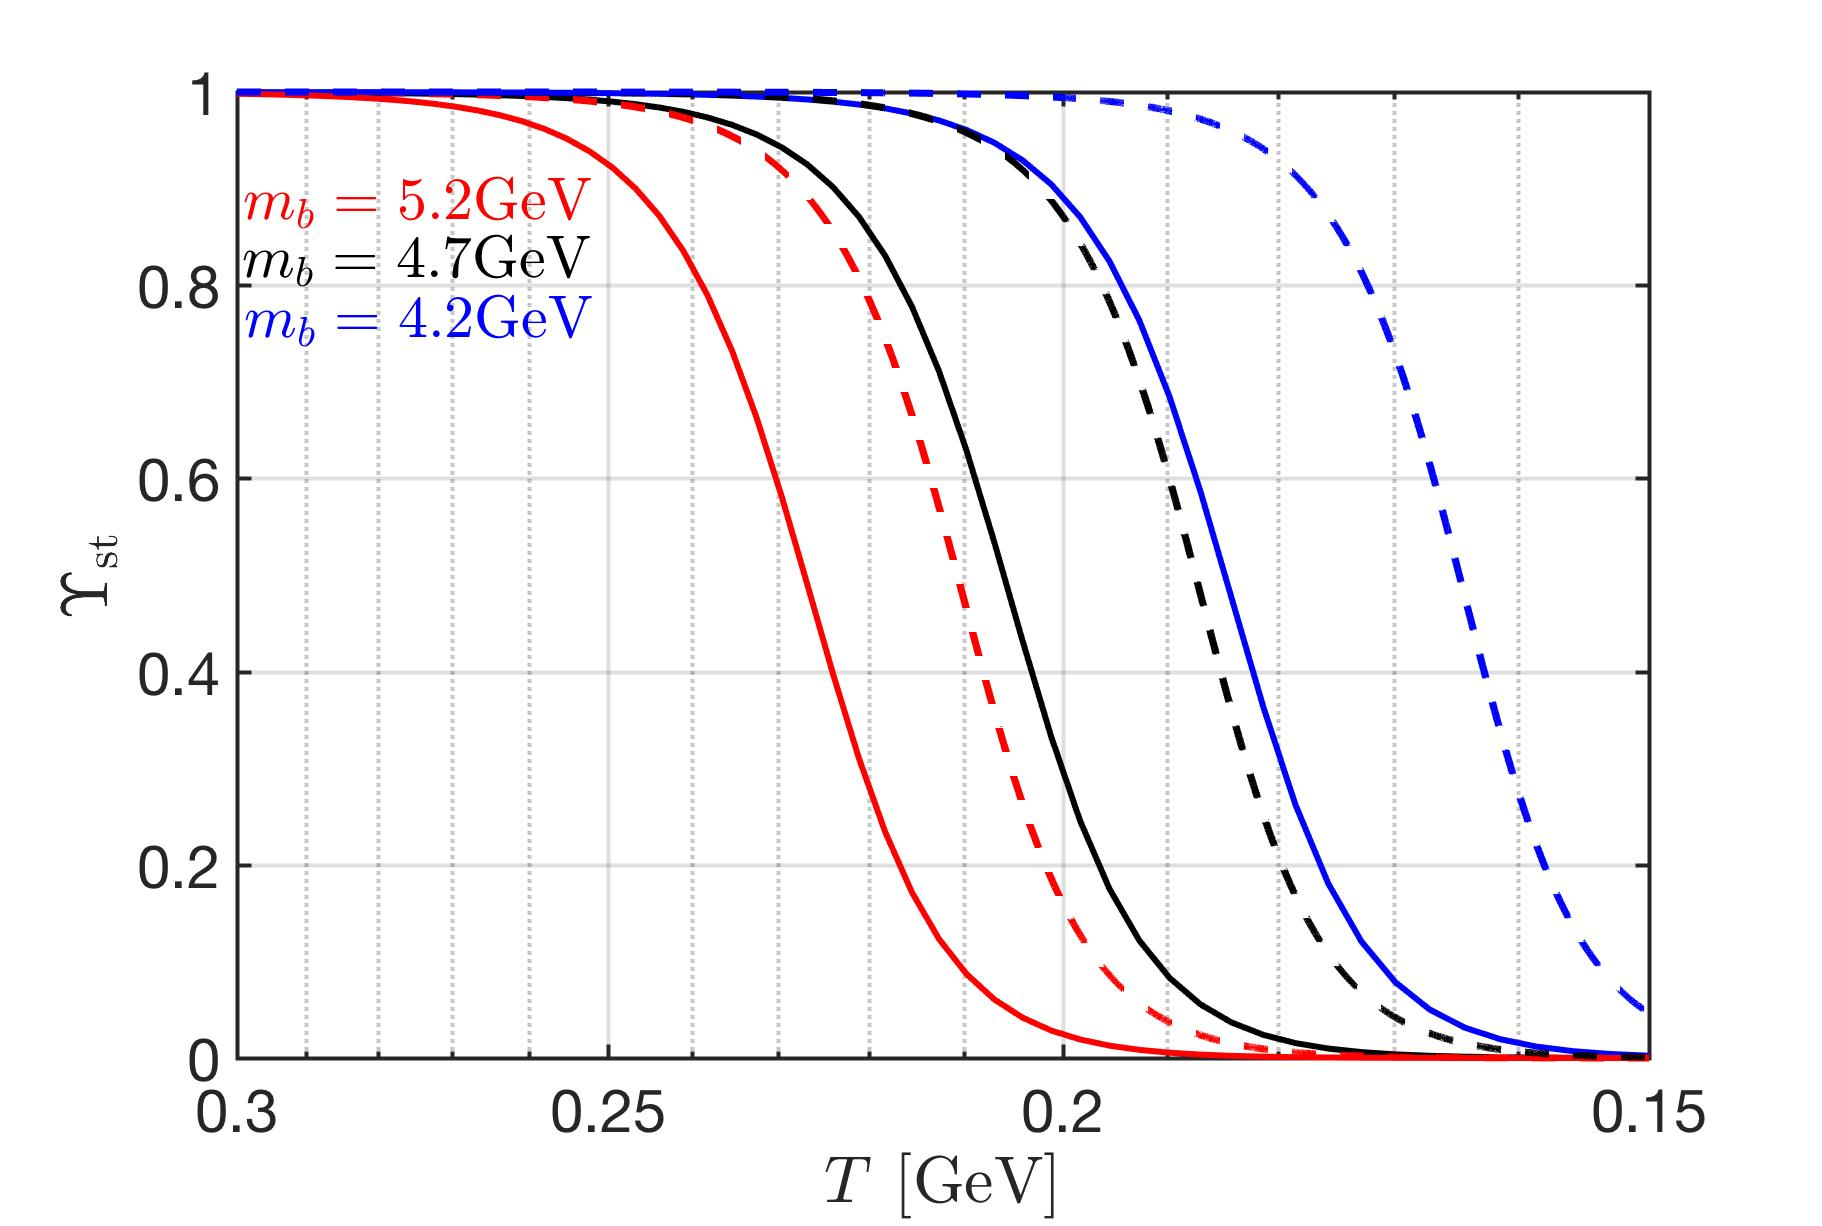
\includegraphics[width=0.8\linewidth]{./plots/BquarkFugacity_tot}}
\caption{Dynamical fugacity of bottom quark as a function of temperature in primordial Universe. Solid line shows bottom quark bound into $B_c$, dashed lines the case of free bottom quark: $m_b=4.2\,\mathrm{GeV}$ (blue), $m_b=4.7\,\mathrm{GeV}$ (black), and $m_b=5.2\,\mathrm{GeV}$ (red). \cccite{Rafelski:2023emw}. \radapt{Yang:2024ret}}
\label{fugacity_bc}
\end{figure}
%%%%%%%%%%%%%%%%%%%%%%%%%%%%%%%%%%%%%%%%%

In~\rf{fugacity_bc} the fugacity of bottom quark\index{bottom quark} $\Upsilon_{\mathrm{st}}$ as a function of temperature, \req{Fugacity_Sol} is shown around the temperature $T=0.3\,\mathrm{GeV}>T>0.15\,\mathrm{GeV}$ for different masses of bottom quarks. In all cases we see prolonged nonequilibrium: This happens since the decay and reformation rates of bottom quarks are comparable to each other as we have noted in~\rf{ReactionTime} where both lines cross. One of the key results shown in~\rf{fugacity_bc} is that the smaller mass of bottom quark slows the strong interaction formation rate to the value of weak interaction decays just near the phase transformation of QGP to HG phase. Finally, the stationary fugacity corresponds to the reversible reactions in the stationary Universe. In this case, there is no arrow in time for bottom quark because of the detailed balance.

We now consider non-stationary correction in expanding Universe allowing for the Universe expanding and thus temperature being a function of time. This leads to a non-stationary correction related to time dependent fugacity in the expanding Universe. 

In general, the fugacity of bottom quark can be written as 
\begin{align}\label{Nonstationary_sol}
&\Upsilon_b=\Upsilon_{\mathrm{st}}+\Upsilon^{\mathrm{non}}_{\mathrm{st}}=\Upsilon_\mathrm{st}\left(1+x\right),\quad x\equiv{\Upsilon_\mathrm{st}^{\mathrm{non}}}/{\Upsilon_\mathrm{st}},
\end{align}
where the variable $x$ corresponds to the correction due to non-stationary Universe. Substituting the general solution \req{Nonstationary_sol} into differential equation \req{Fugacity_Eq0}, we obtain
\begin{align}\label{Nonstationary_eq}
\frac{dx}{dt}=-x^2\frac{\Upsilon_\mathrm{st}}{\tau_{source}}&-x\left[\frac{1}{\tau_{eff}}+3H-\frac{1}{\tau_T}\right]-\left[\frac{d\ln\Upsilon_\mathrm{st}}{dt}+3H-\frac{1}{\tau_T}\right],
\end{align}
where the effective relaxation time $1/\tau_{eff}$ is defined as
\begin{align}
\frac{1}{\tau_{eff}}\equiv\left[\frac{2\Upsilon_\mathrm{st}}{\tau_{source}}+\frac{1}{\tau_{decay}}+\frac{d\ln\Upsilon_\mathrm{st}}{dt}\right].
\end{align}

%%%%%%%%%%%%%%%%%%%%%%%%%%%%%%
\begin{figure} 
\centerline{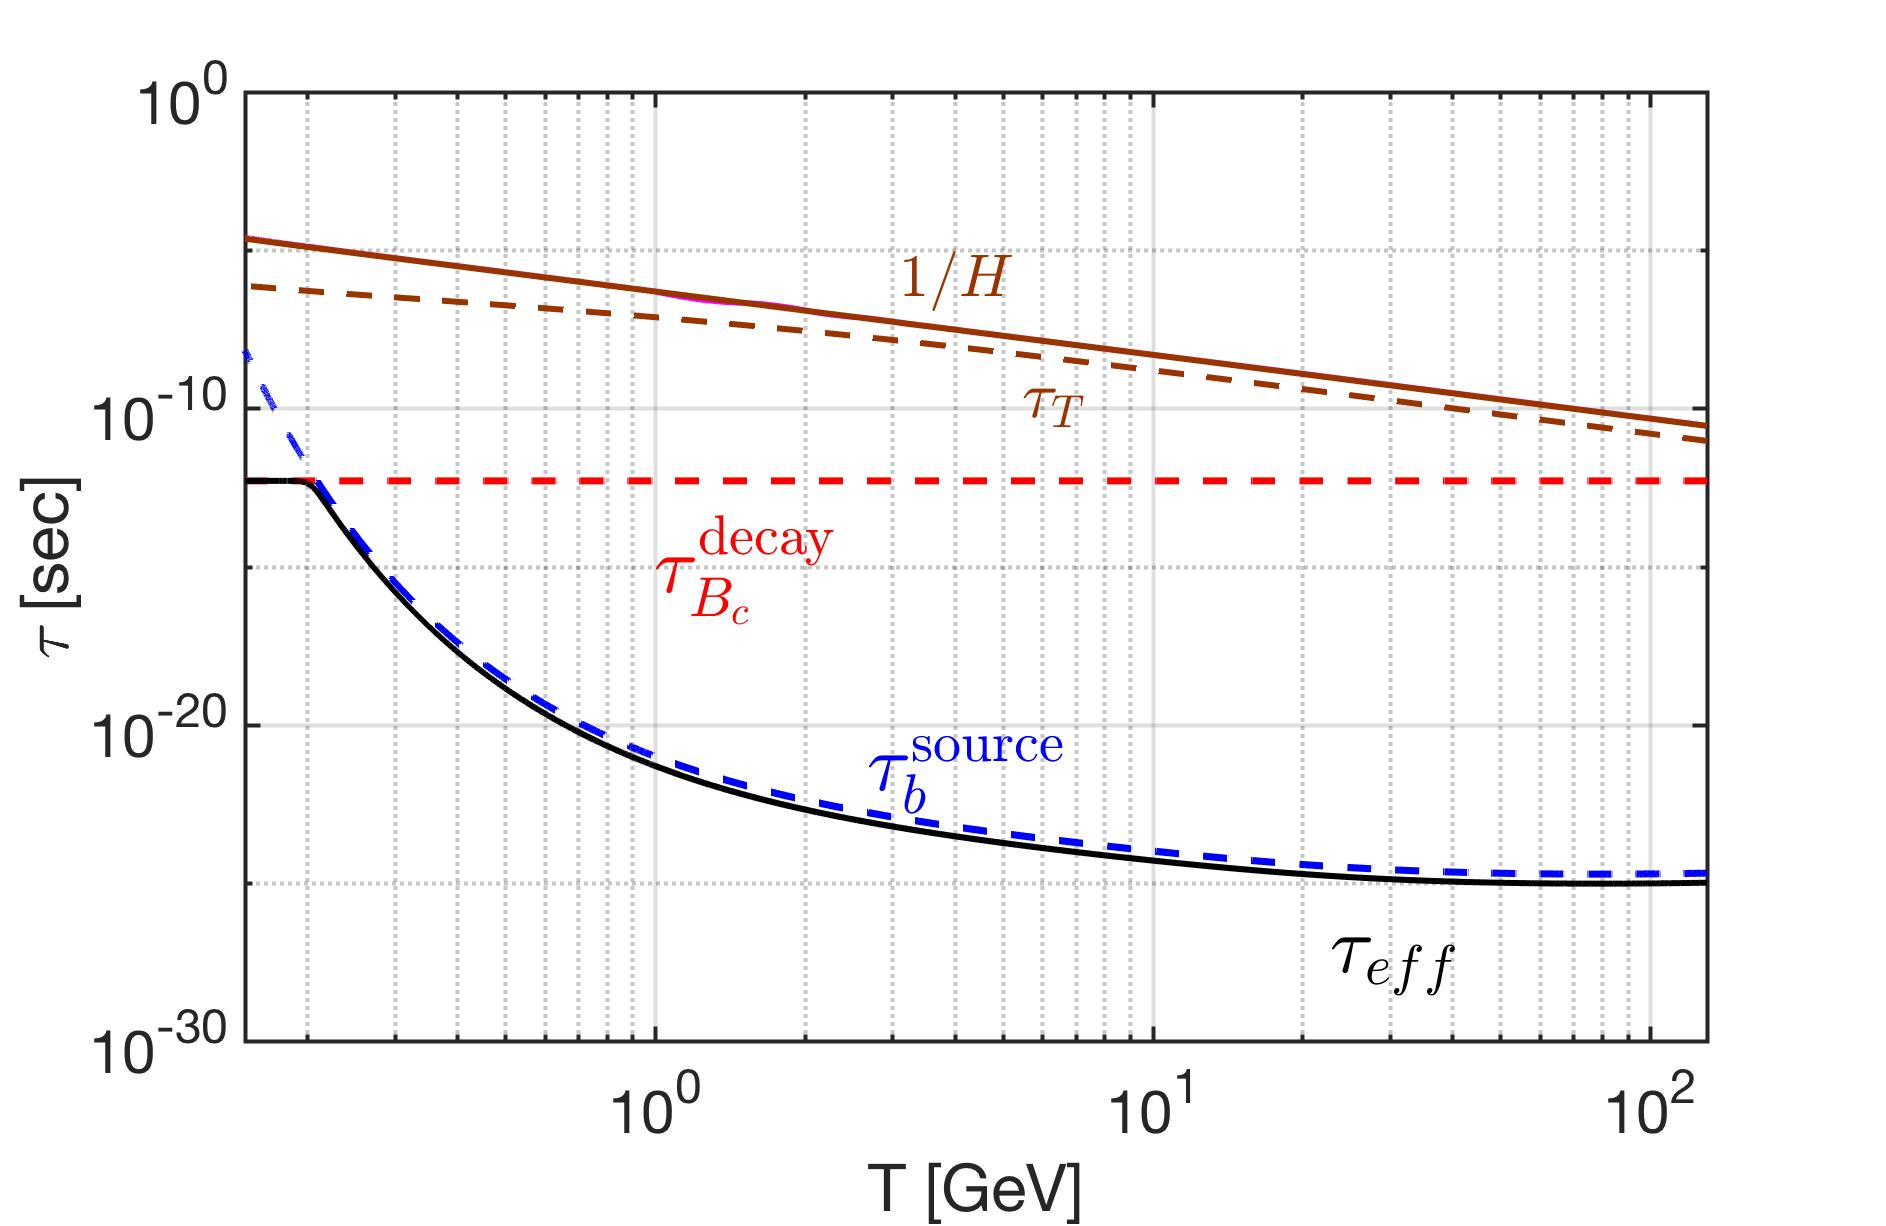
\includegraphics[width=0.8\linewidth]{./plots/Tau_RelaxationTime002}}
\caption{The effective relaxation time $\tau_{eff}$ as a function of temperature in the primordial Universe for bottom mass $m_b=4.7$\,GeV. For comparison, we also plot the vacuum lifespan of $B_c$ meson $\tau_{B_c}^{decay}$ (red dashed-line), the relaxation time for bottom production $\tau^b_{source}$ (blue dashed-line), Hubble expansion time $1/H$(brown solid line) and relaxation time for temperature cooling $\tau_T$ (brown dashed-line). \radapt{Yang:2024ret}}
\label{RelaxationTime_eff}
\end{figure}
%%%%%%%%%%%%%%%%%%%%%%%%%%%%%%%%%

In~\rf{RelaxationTime_eff} we see that when temperature is near to $T=0.2\GeV$, we have $1/\tau_{eff}\approx10^{7}H$, and $1/\tau_{eff}\approx10^5/\tau_T$. In this case, the last two dilution terms in \req{Nonstationary_eq}  are small compared to $1/\tau_{eff}$ and can be neglected. The differential equation becomes
\begin{align}\label{nonstationary_eq}
\frac{dx}{dt}=-\frac{x^2\,\Upsilon_\mathrm{st}}{\tau_{source}}&-\frac{x}{\tau_{eff}}-\left[\frac{d\ln\Upsilon_\mathrm{st}}{dt}+3H-\frac{1}{\tau_T}\right]
\,.
\end{align}

To solve the variable $x$ we consider the case $dx/dt,x^2\ll1$ first; we neglect the terms $dx/dt$ and $x^2$ in \req{nonstationary_eq}, then solve the linear fugacity equation. We will establish that these approximations are justified by checking the magnitude of the solution. Neglecting terms $dx/dt$ and $x^2$ in \req{nonstationary_eq}, we obtain
\begin{align}
x\approx\tau_{eff}\left[\frac{d\ln\Upsilon_\mathrm{st}}{dt}+3H-\frac{1}{\tau_T}\right].
\end{align}
It is convenient to change the variable from time to temperature. For an isentropically-expanding Universe, we have
\begin{align}\label{tau_H}
\frac{dt}{dT}=-\frac{\tau^\ast_H}{T},\qquad \tau^\ast_H=\frac{1}{H}\left(1+\frac{T}{3g^s_\ast}\frac{dg^s_\ast}{dT}\right).
\end{align}
In this case, we have
\begin{align}
x=\tau_{eff}\left[\frac{1}{\Upsilon_\mathrm{st}}\frac{d\Upsilon_\mathrm{st}}{dT}\frac{T}{\tau^\ast_H}+3H-\frac{1}{\tau_T}\right].
\end{align}
Finally, we can obtain the non-stationary fugacity\index{fugacity} by multiplying the fugacity ratio $x$ with $\Upsilon_\mathrm{st}$, giving \index{bottom quark! non-stationary fugacity}
\begin{align}
\Upsilon_{\mathrm{st}}^{\mathrm{non}}
&\approx\left(\frac{\tau_{eff}}{\tau^\ast_H}\right)\left[\frac{d\Upsilon_\mathrm{st}}{dT}T-\Upsilon_{\mathrm{st}}\left(3H\tau^\ast_H-\frac{\tau^\ast_H}{\tau_T}\right)\right].
\end{align}

In~\rf{NonFugacity} we plot the non-stationary $\Upsilon^{\mathrm{non}}_\mathrm{st}$ as a function of temperature. The non-stationary fugacity $\Upsilon^{\mathrm{non}}_\mathrm{st}$ follows the behavior of $d\Upsilon_{\mathrm{st}}/dT$, which corresponds to the irreversible process in the expanding Universe. 

The irreversible nonequilibrium process creates the arrow in time for bottom quarks evolution in the Universe. The relatively large value of Hubble time (relatively slow expansion) is suppressing the value of the non-stationary fugacity resulting in the small $\mathcal{O}\sim10^{-7}$ effect. On one hand this shows that  neglecting $dx/dt,x^2\ll1$ is a good approximation for obtaining the non-stationary fugacity in the primordial Universe. On the other hand this also means that chemical non-stationary effects near to hadronization of bottom quarks could be too weak to allow sufficient baryogenesis.


%%%%%%%%%%%%%%%%%%%%%%%%%%%%%%%%%%%
\begin{figure}
\centerline{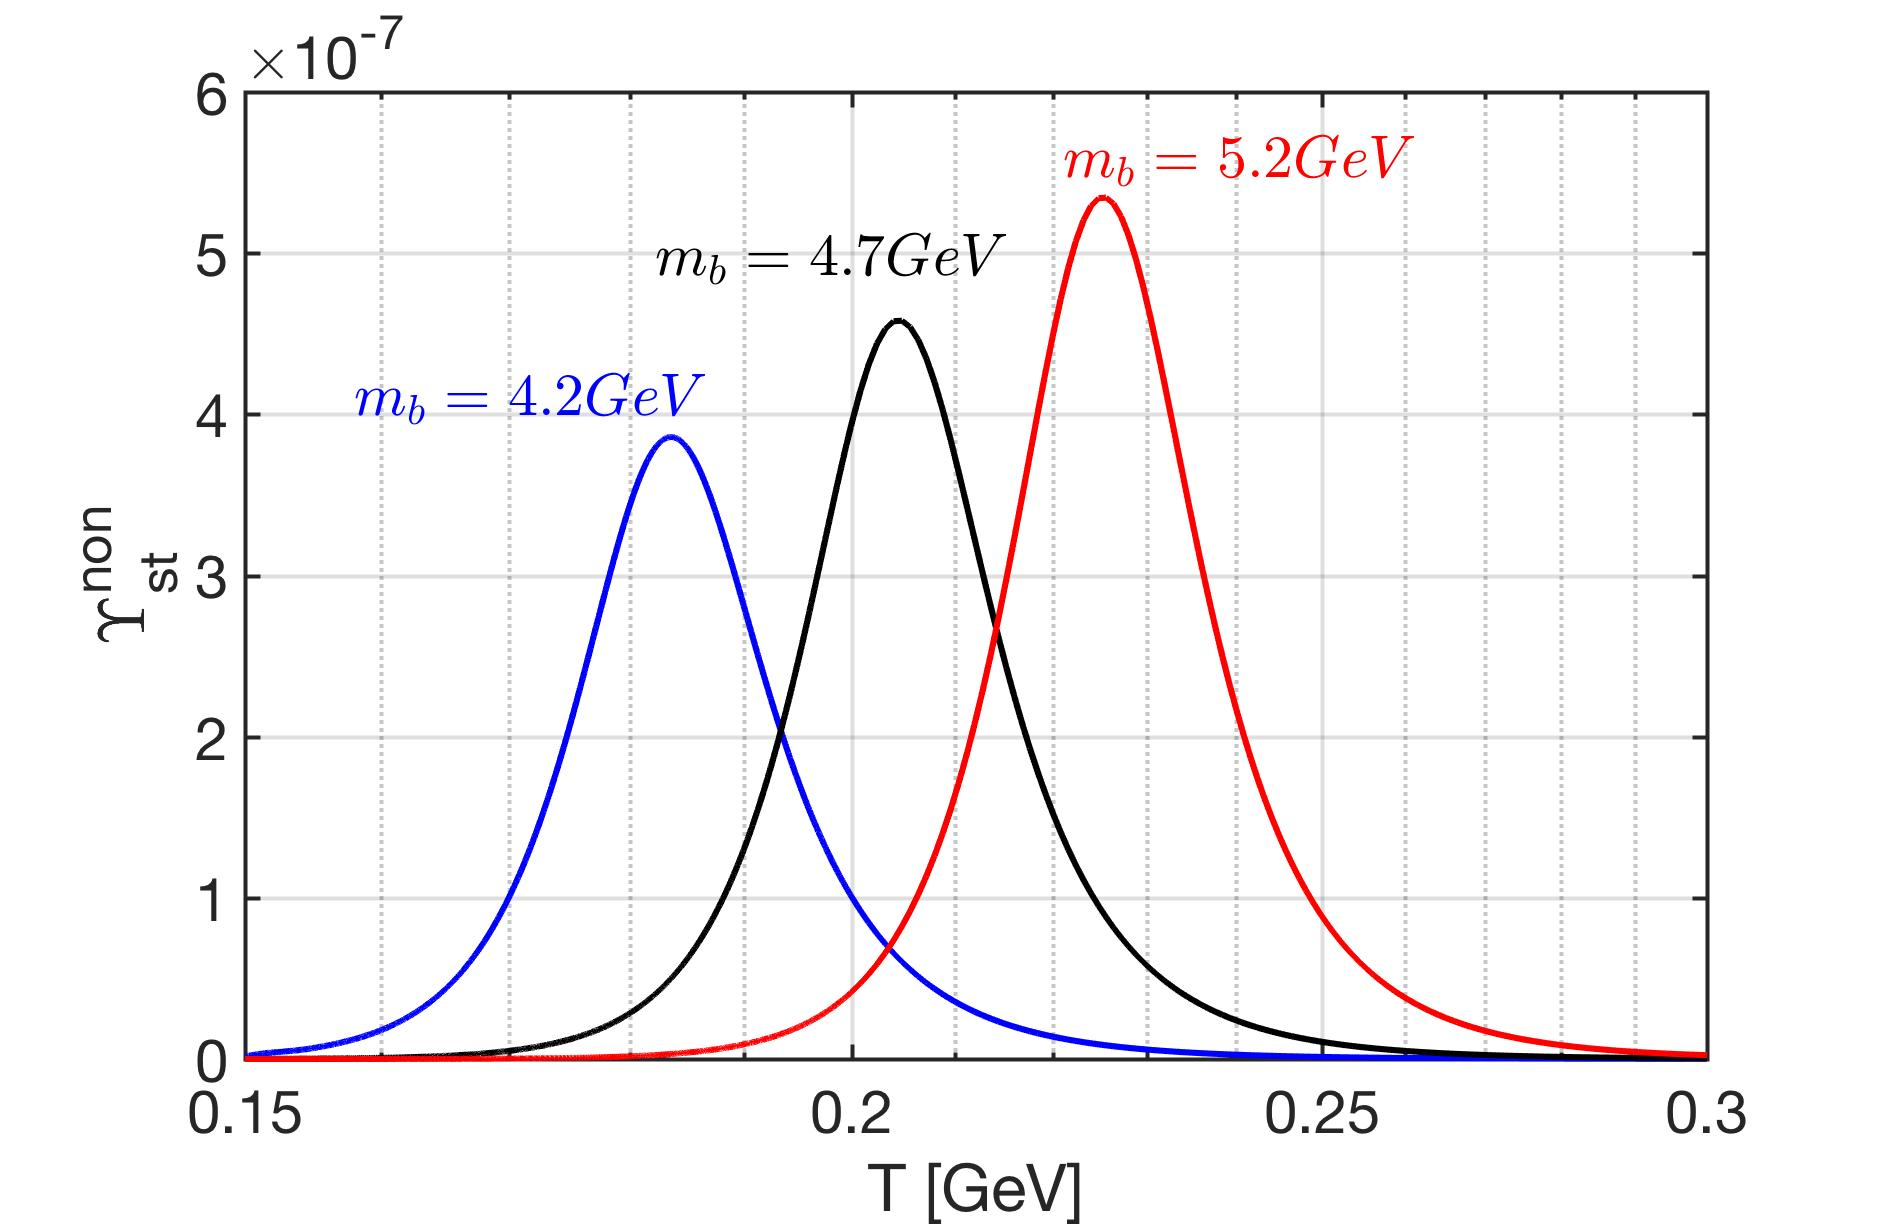
\includegraphics[width=0.8\linewidth]{./plots/NonstationaryFugacity}}
\caption{The non-stationary fugacity $\Upsilon_\mathrm{st}^{\mathrm{non}}$ as a function of the Universe $T$ for three different bottom masses $m_b=4.2\,\mathrm{GeV}$ (blue), $m_b=4.7\,\mathrm{GeV}$ (black), and $m_b=5.2\,\mathrm{GeV}$ (red). \radapt{Yang:2024ret}}
\label{NonFugacity}
\end{figure}
%%%%%%%%%%%%%%%%%%%%%%%%%%%%%%%%%%%%%%
 

%%%%%%%%%%%%%%%%%%%%%%%%%%%%%%%%%%
\para{Is there enough bottom flavor to matter?} Considering that FLRW-Universe evolves\index{cosmology!FLRW} conserving entropy, and that baryon and lepton numbers following on the era of matter genesis is conserved, the current day baryon $B$ to entropy $S$, $B/S$-ratio must be achieved during matter genesis. The estimates of present day baryon-to-photon density\index{baryon!per photon ratio} ratio $\eta_\gamma$ allows the determination of the present value of baryon per entropy\index{baryon!entropy ratio} ratio \cite{Fromerth:2012fe,Rafelski:2019twp,Letessier:2002ony,Fromerth:2002wb}:
\begin{align}
\left(\frac{B}{S}\right)_{t_0}\!\!\!\!=\eta_\gamma\left(\frac{n_\gamma}{\sigma_\gamma+\sigma_\nu}\right)_{\!t_0}\!\!\!\!=(8.69\pm0.05)\!\!\times\!\!10^{-11},
\end{align}
where the subscript $t_0$ denotes the present day value, where $\eta_\gamma=(6.14\pm0.02)\times10^{-10}$~\cite{ParticleDataGroup:2022pth}  is used here. Here we consider that the Universe today is dominated by photons and free-streaming  low mass neutrinos~\cite{Birrell:2012gg}, and $\sigma_\gamma$ and $\sigma_\nu$ are the entropy density for photons and neutrinos, respectively. 
 
In chemical equilibrium\index{chemical equilibrium} the ratio of bottom quark\index{bottom quark} (pair) density $n_b^{th}$ to entropy density\index{entropy!density} $\sigma=S/V$ just above the quark-gluon hadronization\index{hadrons!hadronization} temperature $T_\mathrm{H}=150\sim160\MeV$ is $n_b^{th}/\sigma=10^{-10}\sim 10^{-13}$, see~\rf{number_entropy_b002}. By studying the bottom density per entropy near to the hadronization temperature and comparing it to the baryon-per-entropy ratio $B/S$, we obtain the abundance of bottom quarks to consider in the proposed matter genesis mechanism.

%%%%%%%%%%%%%%%%%%%%%%%%%%%%%%%%
\para{Example of bottom-catalyzed matter genesis}
Given that the nonequilibrium non-stationary component of bottom flavor arises at a relatively low QGP temperature, {\color{black}this Sakharov condition Eq.~(\ref{Sakharov}) is available around QGP hadronization.\index{Sakharov conditions!baryogenesis}} Let us now look back and see how different requirements are fulfilled
%%%%%%%%%%%%%%%%%%%%%%%%%%%%%%%%%%%%
\begin{itemize}
\item
 We have demonstrated non-stationary conditions with absence of detailed balance: The competition between weak interaction decay and the strong interaction gluon fusion process is responsible for driving the bottom quark departure from the equilibrium in the primordial Universe near to QGP hadronization condition around the temperature $T=0.3\sim0.15\GeV$ as shown in~\rf{fugacity_bc}. Albeit small there is clear non-stationary component required for baryogenesis, see~\rf{NonFugacity}.
%%%%%%%%%%%%%%%%%%%%%%%%%%%%%%%
\item Violation of $CP$\index{CP violation} asymmetry were observed in the amplitudes of hadron decay including neutral B-mesons, see for example~\cite{LHCb:2019jta,LHCb:2020vut}. The weak interaction $CP$ violation\index{CP violation}\index{CKM matrix} arises from the components of Cabibbo-Kobayashi-Maskawa (CKM) matrix associated with quark-level transition amplitude and $CP$-violating phase. There is clear coincidence of non-stationary component of bottom yield with the bottom quark $CP$ violating decays of preformed $\mathrm{B}_x$ meson states, $x=u,d,s,c$~\cite{Karsch:1987pv,Brambilla:2010vq,Aarts:2011sm,Brambilla:2017zei,Bazavov:2018wmo,Offler:2019eij}. The exploration of the here interesting $CP$ symmetry breaking in B$_c(b\bar c)$ decay is in progress~\cite{ParticleDataGroup:2022pth,Tully:2019ltb,HFLAV:2019otj}.
\item
We do not know if there is baryon conservation\index{baryon!conservation} violating process in which one of the heavy QGP particles is participating. However, if such a process were to exist it is likely, considering mass thresholds, that it would be most active in the decays of heaviest standard model particles. It is thus of considerable interest to study in lepton colliders baryon number non conserving processes at resonance condition. Such a research program will additionally be motivated by our demonstration of an extended period of baryogenesis in the primordial Universe. 
\end{itemize}

%%%%%%%%%%%%%%%%%%%%%%%%%%%%%%%%%%%%%%%%%%%%%%
\para{Circular Urca amplification}
The off equilibrium non-stationary behavior of bottom quarks near the temperature range $T=0.3\sim0.15\GeV$ can provide the environment for baryogenesis to occur in the primordial-QGP hadronization era. The non-stationary effects of interest, as we saw, are small. However there is an additional amplifying factor. 
 
 Let us consider the scenario where all bottom quarks are confined within $B_c^\pm$ meson. In this case, we know that the $B_c^\pm$ decay in the primordial-QGP has $CP$ violating component. We also know as shown above that there is a small  irreversible fraction of the evolving fugacity. Let us assume in addition that  there is a tiny baryon number breaking decay of the $B^\pm_c$ meson. A baryon symmetry will be accompanied by the asymmetry between leptons\index{lepton} and anti-leptons assuming $B-L=0$ baryon number violating processes.

The heavy $B_c^\pm$ meson decay into multi-particles in `cold' $T=0.3\sim0.15\GeV$ plasma is  naturally associated with the irreversible process. This is because after decay the daughter particles can interact with plasma and distribute their energy to other particles and reach equilibrium with the plasma quickly. In this case the energy required for the inverse reaction to produce $B_c^\pm$ meson is difficult to overcome and therefore we have an irreversible process for multi-particle decay in plasma.

This said we note that the rapid $B_c^\pm$ decay and bottom reformation speed at picosecond scale assures that there are millions of individual microscopic processes involving bottom quark production and decay before and during the hadronization epoch of QGP. In this case, we have a so-called Urca (after Urca Casino in Rio de Janeiro, Brazil) process for the bottom quark, i.e. a cycling reaction in which we have a multitude of circular production and decay processes involving $B_c^\pm$ meson. 

The Urca process is a fundamental physical process and has been studying the realms of in astrophysics and nuclear physics. In our case, for bottom quark as a example: at low temperature, the number of bottom quark cycling can be estimated as
\begin{align}
\left.\mathrm{C_{cycle}}\right|_{T=0.2\mathrm{GeV}}=\frac{\tau_H}{\tau_{B_c}}\approx2\times10^7,
\end{align}
where the lifespan of $B_c^\pm$ is $\tau_{\mathrm{B}_c}\approx0.51\times10^{-12}\,\mathrm{s}$ and at temperature $T=0.2\GeV$ the Hubble\index{Hubble!time} time is $\tau_H=1/H=1.272\times10^{-5}\,\mathrm{s}$. 

The Urca process\index{Urca process!baryogenesis} plays a significant role by potentially amplifying any small and currently unobserved violation of baryon number associated with the bottom quark. The small baryon asymmetry is enhanced by the Urca-like process with cycling ${\tau^\ast_H}/{\tau_\ast}$ in the primordial Universe. This amplification helps achieving the required baryogenesis strength.
